\documentclass[shuuron]{kuee}
\usepackage[dvipdfmx]{graphicx}
\usepackage{lineno,hyperref}
\usepackage{kueecite}
\usepackage{url}

\title{心理カウンセリングの\\品質向上を支援する\\視覚的分析に関する研究}
\author{上辻智也}
\professor{小山田 耕二 教授}
\course{京都大学大学院工学研究科}
\department{電気工学専攻}
\date{平成30年2月1日}

%%% 本文
\begin{document}
\maketitle
\tableofcontents


%%%序論
\chapter{序論}



心療において,カウンセラーは心身症やストレスからくる身体症状をもつ患者やクライエント(以降,「患者やクライエント」を「クライエント自身」と統一する)に対してカウンセリングを行う.1991年に日本心身医学会が「心身症とは,身体疾患の中で,その発症や経過に心理社会的因子が密接に関与し,器質的ないし機能的障害が認められる病態をいう.ただし,神経症やうつ病など,他の精神障害に伴う身体症状は除外する」と定義した\cite{shinshinigaku}.その後、心身症はストレスとの深い関連が指摘された病態であると認知され,今日まで広く研究されてきた.クライエントの関心、いわゆる「対人関係上の問題」にカウンセラーが自身の関心を向けて傾聴するということがカウンセリングの基本である\cite{zokad}.

%そこで,心理カウンセリングにおいて, カウンセラーは,主にストレスの原因による物理的な症状に悩むクライエントに対してカウンセリングを提供している.カウンセリングの会話は音声ないし動画として記録され,後述するカウンセラー指導・事例検討の目的で役立てられているが,クライエントのプライバシーの関係上、実際の事例検討やカウンセラー教育の場では,それを書き起こした逐語録を用いることが多い.




%%品質の定義


カウンセリングの品質向上のために、会話記録を基に熟練したカウンセラーが初心者のカウンセラーに対してアドバイスを行う熟練したカウンセラーが初心者のカウンセラーに指導する機会としての事例検討会が行われている。武藤ら\cite{武藤清栄2007人間関係やコミュニケーション障害による生産性の低下}は医療に携わる人間のコミュニケーション能力の低下がカウンセリングを含むサービス業としての医療の品質の低下につながるとしている。植田ら\cite{植田一博2006会話の分析とモデル化}はカウンセリング中の非言語行動から品質の導出を試みたが、テキストからはそのような非言語行動が読めない。

今回取り扱うヨーガ療法において鎌田ら\cite{Darshana}によれば、カウンセリングの目的はクライエントの認知を修正することであるが、初心者のカウンセラーはクライエントの関心に自分の関心を傾聴することが困難であり、したがってクライエントの認知を修正する段階までいくのが困難である。
そこで本研究で述べるカウンセリングの品質とは、下記の2つの項目によって構成されるものとする。
\begin{itemize}
  \item カウンセラーの関心がどのくらいクライエントの関心に傾聴されているか
  \item クライエントの認知の修正がどのくらい進行しているか
\end{itemize}


熟練したカウンセラーから初心者のカウンセラーへの指導をスーパービジョンと呼び、指導する側である熟練したカウンセラーはスーパーヴァイザー、指導される側である初心者のカウンセラーはスーパーヴァイジ―と呼ばれるが、クライエントと初心者のカウンセラーとのカウンセリングの会話記録を基に熟練したカウンセラーが初心者のカウンセラーに対して指導を行う,というのがスーパービジョンの流れである.
カウンセリングの会話記録はカウンセラー教育・事例検討を目的として,音声ないし動画が撮影される.しかし,プライバシーの関係上,それらを手で書き起こしたテキストの逐語録にして用いることが多い.そのため,熟練したカウンセラー達が会話の流れを文字で読むだけでは,カウンセリング内容の分析において、どのような質問からどのような回答が発せられたかという理解が,十分に行えていない可能性がある.

%具体的な理由
%・例えば:一長一短では治らない.こんなに閉じられた質問をしていたのかという実感が沸かない.

また,同じクライエントとカウンセラーが複数回カウンセリングを行っていくと,会話のテキストデータは膨大となり,全てのカウンセリング中,どのカウンセリングにおいてクライエントの認知の修正がどこまで進んでいるかを把握することは困難になる。%,複数のカウンセラーで客観的に把握するのは今日行われていない.ヨーガ療法事例検討会においても,全てのカウンセリングにおいては事例の検討を複数カウンセラーでは行われていない.

% その中で,スーパーヴァイジーは自分の関心でカウンセリングを進めてしまいがちで,自分の中で作り上げた解釈内容をクライエントに確認するための「閉じられた質問(closed-ended question)」を多用する傾向が顕著にみられる.

以上から,品質向上のために、カウンセリングの品質の定義として本研究で前述した2点を直感的な把握を支援することが必要であり、そのためにカウンセリング会話内容から適切な手法でこれら2点を視覚的に分析を行えるシステムをつくることが本研究の目的である。
% \begin{itemize}
%
%   \item
%   スーパーヴァイジーがどのような質問をして,それに対してクライエントがどのように反応しているのか
%   \item カウンセリングによって、クライエントの認知の修正がどのくらい進んだか
% \end{itemize}


%・カウンセラー

% そこで心理カウンセリングの会話書き起こしテキストデータから会話内容を可視化することで,心理カウンセリングの品質向上を支援することができるのではないかと本研究では考えた.

ここで,本研究では,「心理カウンセリングの品質向上を支援する視覚的分析」の要素として次の2つに着目する.
\begin{itemize}
  \item 心理カウンセリングにおいてカウンセラーの関心がどのくらいクライエントの関心に傾聴されているかの評価を支援する「会話の流れの視覚的分析」
  \item 心理カウンセリングにおいてクライエントの認知の修正すなわち回復状況の評価を支援する「認知の修正の視覚的分析」
\end{itemize}

% ただしここでいう習熟度とは,後述する「カウンセラーがどのくらい開かれた質問と閉じられた質問を使い分けられるか」と定義する.

% 本論文では,「カウンセリングの品質向上への支援」を以下のように定義する.
% ・熟練したカウンセラーからのアドバイスを含む,初心者のカウンセラーのカウンセリングの質問の品質向上への支援
% ・クライエントのクライエントの認知の修正をカウンセラーが把握することへの支援

\subsubsection{会話の流れの視覚的分析}

%%%%%%%%%%%習熟度の定義



質問に対する回答として発せられるクライエントの関心、いわゆる「対人関係上の問題」にカウンセラーが自身の関心を向けて傾聴するのに苦戦しているという問題がある.鎌田ら\cite{Darshana}によれば、まずカウンセラーは自分のクライエントに対する解釈をクライエントに押し付けがちになり、カウンセラーがクライエントよりも多く喋ってしまう傾向にある。
また、カウンセラーの質問内容は,大きく次の2種類に分けられている.YesまたはNoで答えられる質問,または短い言葉だけで答えられるような質問は「閉じられた質問」または「閉ざされた質問」(Closed-ended Question)と呼ばれている.これに対し,5W1H「いつ」「どこで」「誰が」「何を」「どのように」「どうした」で問うような質問は「開かれた質問」(Open-ended Question)と呼ばれている.熟練したカウンセラーによれば,クライエントが何に問題意識を感じているかに対してカウンセラーの関心を傾聴するには,カウンセラーは「閉じられた質問」よりも「開かれた質問」をしたほうがよいとされている\cite{ivey}.しかし初心者のカウンセラーは「閉じられた質問」の割合が多く,クライエントが何に問題意識を感じているかに対してうまくカウンセラーの関心を傾聴できないケースが比較的多いとされている.

% 「対人関係上の問題」に注意を向けるということがカウンセリングの基本であるので,このようにカウンセラーの関心でクライエントを誘導してしまうことはよくないとされている.カウンセラーの事例検討会において,熟練したカウンセラー達が会話の流れを文字で読むだけでは,カウンセリング内容の分析が十分に行えていなかった.

このように,初心者のカウンセラーは「閉じられた質問」を多く用いる傾向にあるので,熟達カウンセラーは,初心者のカウンセラーが「閉じられた質問」だけでなく「開かれた質問」も使いこなせるように教育したいと考えている.しかし,熟練したカウンセラー達が会話の流れを文字で読むだけでは,カウンセリング内容の分析において、どのような質問からどのような回答が発せられたかという理解が,十分に行えていない可能性がある.そこで,初心者のカウンセラーがどのような質問をして,それによってクライエントからどのような回答が発せられたのか,適切な手法で可視化されることが望まれていた.

キーワードベースでの会話内の話題の可視化は Danielle Albersら\cite{angus2012conceptual}が行っていたが、話者を2人に絞り、どのような質問からどのような回答が得られるかという質問と回答の対応関係はこの可視化手法では解決されない。

そこで本研究では,クライエントと初心者のカウンセラーとの会話の流れを,時間軸に沿って可視化するシステムを開発することで、カウンセラーの関心がどのくらいクライエントの関心に傾聴されているかについてカウンセラーにより理解を深めさせる.本提案システムは熟練したカウンセラーをユーザーとして想定した.熟練したカウンセラーから初心者へのカウンセリング指導において重要なことは,初心者のカウンセラーがクライエントにどのような質問を投げかけるかによって,初心者のカウンセラーがクライエントからどのような「対人関係上の問題」に対してカウンセラーの関心を傾聴したかである.それが一目見てすぐにわかるようになることが,「会話の流れの視覚的分析」によって期待されることである.%システムをWeb上に載せることによって,同じ会話データを持っているだけで遠隔のユーザーと同様の可視化を共有することが期待される.



% クライエントの会話内容としては,次章で詳しく述べるどのタスク領域(仕事,交友,愛)に属するのか,カウンセラーの質問としては,内容が「開かれた質問」なのかまたは「閉じられた質問」なのかを分類表示できることが必要である.



\subsubsection{認知の修正の視覚的分析}

% クライエントは,多くの場合,より多くのクライエントの認知の修正は心理カウンセリングに進行し,「アクションの他人の話をクライエントに自分自身を行っている」.2「彼らが行っていることを言動について話す」の割合として言いる.言い換えれば,「あなた自身の言動を変えるのではなく,相手の言動を変えることに関心がある場合は,認知修正が進んでいる」[1].したがって,本研究では適切なカウンセリングの会話データから,「クライエントの言動」と「クライエントの言動を」分類し,結果を可視化することにより,クライエントの認知の修正の度合いを把握することができる,と考えた.

%一連の文章の中から,場面ごとに誰が誰に言動を起こしたか把握したい,会話文や物語の人間関係を想起する必要がある場面がある.たとえば
心理カウンセリングにおいて,クライエントは「他人がクライエント自身に行った言動」ではなく,「自分が行った言動」の話をカウンセリング中にする割合が多いほど,クライエントの認知の修正が進行しているといわれている.つまり、「相手の言動を変えることより,自分の言動を変えていくことに関心がある方が,認知の修正が進んでいる」\cite{zokad}とされている.また,クライエントの回答として「クライエントの身の回りの人の言動」に関する発言よりも「クライエント自身の言動」に関する回答が発せられた方が,クライエントの認知の修正が進行しているとされている.
しかし、同じクライエントとカウンセラーが複数回カウンセリングを行っていくと,会話のテキストデータは膨大となり,全てのカウンセリング中,どのカウンセリングにおいてクライエントの認知の修正がどこまで進んでいるかを把握することは困難になる。この問題を解決するために、「クライエントの身の回りの人の言動」か「クライエント自身の言動」かを、会話データを元に可視化することで,クライエントの認知の修正の理解を深めさせる.

ヴァンハム\cite{van2009mapping}らがユーザーによって指定された「BのA」および「AおよびB」の関係を有向グラフで表現した可視化研究が存在している.しかし,接続詞や前置詞ベースで単語をつなげている彼らのシステムから,本研究では誰が誰に対して言動を発したかを知ることは不可能である.

% 以上のように,どのような場面で誰が誰に言動したかを文書から抽出することが求められている.それに対し本研究では,誰が誰にどのような言動をとったかを時系列で可視化することで,上記のニーズを満足できるのではないかと考えた.このような要求に対し,本研究では誰が誰に言動したかという人間関係図を時系列にそった可視化を試みた.

したがって,本研究では心理カウンセリング会話中に登場する人々の間でどのような言動が誰から誰へ発せられたかを可視化する人間関係図を用いることで、会話データの可視化を試みた.

本論文の構成は次の通りである.第1章は,本論文の序論である.第2章では,本論文の関連研究を挙げる.また,提案システムの開発にあたり必要になってくるカウンセリングの基礎事項について説明する.第3章では,心理カウンセリングにおいて初心者のカウンセラーの習熟度の評価を支援する「会話の流れの視覚的分析」について述べる.第4章では,心理カウンセリングにおいてクライエントの認知の修正すなわち回復状況の評価を支援する「認知の修正の視覚的分析」について述べる.第5章では,本論文の結論と本研究が抱える今後の課題について述べる.

%


%
%   特に心理共同でunseling, カウンセラーは,主にストレスの原因による物理的な症状に心身クライエントやクライエントとのカウンセリングを提供している.一般的には,初心者のカウンセラーは,認知特性とクライエントによる内部問題の難易度回し関心を持っている.
%   初心者のカウンセラーは,自分の関心に合わせて心理カウンセリングを続行する傾向があり,および周波数を使用している「クローズド・エンド型の質問(クライエントは答えることができ, 『いいえはい』または『』)」クライエントのために,人の心の中で作成された解釈を確認する.初心者のカウンセラーはメイククライエントの認識こだわり答えを得ることができない
% しばしば,初心者のカウンセラーのはい/いいえの質問
%   これとは対照的に,専門家のカウンセラーがカウンセリングの内容に関する初心者のカウンセラーのための助言に教育訓練の機会を提供する.熟練したカウンセラーは,そのため,初心者のカウンセラーが「オープンエンドの質問(5W1Hによる質問)」を自由に使用することができる教育する必要がある.しかしながら, なぜなら,プライバシーの問題のため,専門家は,心理カウンセリングの実際の音声データを取得することはできない. だから, いつも監督に,専門カウンセラーは,カウンセリングで音声表記の直接書き起こしテキストと見て,初心者のカウンセラーのために誰かを教育する.
%   しかし,書き起こし産物の文書 テキストデータが 心理カウンセリングにおける会話の大規模かつ複雑で,スーパーヴァイザは各データを参照しながら,初心者のカウンセラーとクライエント間の特性との会話の状況を抽出することは非常に困難である.この問題を改善するために,本研究では,会話データの可視化が有効であると思われることを検討してください.したがって,本研究では,初心者のカウンセラーによる各質問のためのクライエントの各回答を可視化するための適切な手法を示すことを検討してください.
%   本研究では,心理カウンセリングに会話の流れを可視化するシステムを提案し,開発した.この提案システムでは,本研究ではAdlerian心理学の基礎を分類し,各カテゴリグループのためのチャートと時間の経過に沿って分布の変動を可視化表音transcriptio中含まれて,n 心理カウンセリングにいる.本研究では,システムの概要とUの結果を示する熟練したカウンセラーによるSER評価.会話の流れの私達の可視化の対象ユーザーは,専門家のカウンセラーである.
%    また,クライエントは,多くの場合,より多くのクライエントの「認知の補正は,」図のように心理カウンセリングに進行し,「アクションの他人の話をクライエントに自分自身を行っている」.2「彼らが行っていることを言動について話す」の割合として言いる.言い換えれば,「あなた自身の言動を変えるのではなく,相手の言動を変えることに関心がある場合は,認知補正が進んでいる」[1].したがって,本研究では適切なカウンセリングの会話データから,「クライエントの言動」と「クライエントの言動を」分類し,結果を可視化することにより,クライエントの認識の変更の度合いを把握することができ,と考えた.
%   上記の要求に応じて,本研究では言動のどのような心理カウンセリング会話中に登場する人々の間で撮影された人間関係のチャートとを組み合わせることの手法で会話データを可視化した.


%%







%%%関連研究
\chapter{関連研究}



%%


%%各論文について倍増

本章では,本研究に関連する先行研究について示し,本研究の位置付けについて明らかにする.本研究では,心理カウンセリングでの会話のテキストデータを扱う上で、時系列に沿って可視化する手法が重要であると考えている.

\section{会話中の話題の可視化に関連する先行研究}

本節では,会話の可視化に関する先行研究について述べ,それらの先行研究に対して,我々の提案手法のうち,「会話の流れの視覚的分析」の位置づけについて説明を行う.

A.Tat\cite{tat2002visualising}は,会話の音声波形の可視化を使用し,その波形履歴が周期的にわかるような可視化の工夫を施した.
またTonyら\cite{bergstrom2007seeing}は,話し手の感情を推測することを目的に,複数のマイクの入力から誰が誰に話しかけているかを可視化した.しかし,A. TatらおよびTonyらの研究は,自然言語処理を使用して,会話のコンテンツカテゴリを可視化していない。本研究対象であるカウンセリングにおいて、彼らの可視化手法から質問と回答の関係を知ることができない.

会話以外においても,物語などにおける話題の推移を可視化している研究は多い.例えば,Eric\cite{taskdriven}は,主題の内容をテキストから統計学的に抽出する手法であるトピックモデリングを用いて,二種類で割ったトピックの時間分布を,上下で分けた非対称層折れ線グラフにより可視化している.本研究では,上部と下部の非対称性の折れ線グラフで絵を描くための可視化技術は,クライエントによって各発話や初心者のカウンセラーについて有用であることを考える.しかし,心理カウンセリングの会話の流れを可視化するために,初心者のカウンセラーによる質問に対するクライエントのどのような応答を聞くことが重要である.また今回プライバシーの問題上,3章にて後述する「自己のタスク」や「スピリチュアルのタスク」を自動抽出するための機械学習に必要な多量のカウンセリング書き起こしテキストは得られていなかったため,トピックモデリングを適用することは出来なかった.Weiwei Cuiら\cite{cui2011textflow}は、話題進化傾向、重要なイベント、キーワード相関関係の3種類の可視化を用いて、トピックの流れを可視化した。しかしこちらの可視化についても、個々の質問についての可視化にそぐわないためカウンセラーの関心の可視化には合わず、また認知の修正の可視化のために登場人物をたくさん列挙するのにも向いていない。またキーワードベースでの会話内の話題の可視化は Danielle Albersら\cite{angus2012conceptual}が行っていたが、話者を2人に絞り、どのような質問からどのような回答が得られるかという質問と回答の対応関係はこの可視化手法では解決されない。

会話中の話題を可視化している研究はまだ少ないが,
伊藤\cite{itoh2010interactive}は,3次元に,ブログのユーザーの関心深いトピックの時系列推移を可視化することができ,システムを開発した.本研究では,クライエントによる会話の情報は,時系列,文章のグループ,および文の数によって3次元データから構成されている.しかし,本研究ではクライエントと初心者のカウンセラーとの会話の流れが色分けして2次元のグラフで可視化することができると考えた.%他の手で,初心者のカウンセラーによって発話の情報を時系列と質問タイプによって2次元データである.

またEL-Assady\cite{el2016contovi}は,円周上にトークカテゴリが並べられたチャート内に発話者の円を置いて移動させることで,発話者が今何のはなしをしているかを発話者の円の座標を用いて視覚的に表した.また発話者が居た位置にその発話量を表す円形を置いて残すことで,発話者の会話カテゴリ履歴がわかるようにした.
しかし,カウンセラーとクライエントのトピック分類が一緒でない限り,彼らの可視化を使用することはできないので,本研究では彼らの可視化からの質問と回答の間の関係を知ることができない.

本研究では,心理カウンセリング内で初心者のカウンセラーの質問とクライエントの回答との対応関係を表現した可視化手法が重要である.本研究ではクライエントと初心者のカウンセラーとの各発言カテゴリーと発言量が同時に可視化出来ていることが望ましいと考えた.この事項については次章で詳しく述べる.


%%
%
% 会話の可視化に関していくつかの先行研究がある.本章では,関連する研究を説明し,本研究の位置づけについて説明する.本研究では,時系列に沿って可視化手法は,心理カウンセリングでの会話の流れテキストデータを扱う上で重要であると考えている.
% Heliang[2]は,Webベースの心理カウンセリングシステムで折れ線グラフと3次元の螺旋構造を用いてクライエントのトピックを可視化した.彼らの研究では,このような多種・多様な心理データを3D グラフで可視化する手法が提案されている.本3D グラフ表示はProcessing プロジェクトを用いて螺旋形状の表示を実
% 現する.また螺旋全体を回転させることで,全体的な傾向や特徴を視覚的に把握することが可能となっている
% 一年間を通じてどのような時期(季節,月)に相談量が多くなっているか,そしてその相
% 談内容の詳細も同時に容易に把握することが可能となっている.
% しかし,本研究では,ビューの時点で,初心者のカウンセラーとクライエントの一対一の会話の流れの可視化と呼ばれる,両方で各発話内容を組み合わせることにより,可視化することが重要である.
%  エリックと技術の二種類[3]で割ったトピックの時間分布のための頂部および底部の非対称層折れ線グラフにより可視化他人.本研究では,上部と下部の非対称性の折れ線グラフで絵を描くための可視化技術は,クライエントによって各発話や初心者のカウンセラーについて有用であると考える.しかし,心理カウンセリングの会話の流れを可視化するために,初心者のカウンセラーによる質問に対するクライエントのどのような応答を聞くことが重要である.
%  伊藤は,3次元[4]座標上に,ブログのユーザーの関心深いトピックの時系列推移を可視化することができ,システムを開発した.本研究では,クライエントによる発話の情報は,時系列,文章のグループ,および文の数によって3次元データから構成されている.他の手で,初心者のカウンセラーによって発話の情報を時系列と質問タイプによって2次元データである.しかし,本研究ではクライエントと初心者のカウンセラーとの会話の流れが色分けして2次元のグラフで可視化することが可能であると考えた.
%   EL-Assady [5]は,カテゴリ別にトーク量を意味する円,トークカテゴリを表す円形のチャートを用いて,話者がどのカテゴリのことをしゃべっているかを表す視覚的な分析手法を開発した.彼らはあなたが話題にしているサークルによって会話を表現した.多人数会話の話者言動パターンを分析するための新しい視覚的分析手法として彼らは,会話の主題景観全体にわたる話し手の動きを追跡するためにトピック空間ビューを提案した.彼らのツールは,スピーチの相互作用や言動パターンに関する仮説を生成し,証明するために,政治学者が会話を探るのを支援することを目的としている.関連するテキストの特徴を抽象化するために,スピーカーの一般的な動作や相互作用,時間の経過に伴うインタラクティブな安定した可視化を探索し,スピーカーの選択に関する詳細な分析を行うためのアニメーション表示を提供している.視覚的沈降法のメタファーを使用することにより,分析者は過去のすべてのスピーカーターンの概要を保持しながら,時間の経過とともに会話の流れの微妙な変化を追跡することができるようになっている.しかし,カウンセラーとクライエントのトピック分類が一緒でない限り,彼らの可視化を使用することは不可能であるので,本研究では彼らの可視化手法からの質問と回答の間の関係を知ることが不可能であると考えている.
%  A.タットは,[6]オーディオの可視化を使用し,本研究では言動を言動履歴の追加で拡張する手法を示すためにしようとした.
% 
 トニー・バーグストロームの可視化は,[7]話し手の感情を推測することが可能で,どのように彼/彼女が会話中に別の話者に接続されている.しかし,A. Tatおよびトニーは,自然言語の手順を使用して,会話のコンテンツカテゴリを可視化していないので,本研究では彼らの可視化からの質問と回答の間の関係を知ることが不可能である.
%  本研究では,このような問題は心理カウンセリングで初心者のカウンセラーによってクライエントから引き出すことが可能である手法として,これらの発話に対応することが重要である.したがって,本研究ではクライエントと初心者のカウンセラーによって発話の各情報をことが望ましいと考えた コンパクトなシングルチャートで可視化することを試みた.
%  カウンセリングについて3.基本的な説明
%  本章で,我々の提案するシステムの開発に必要なカウンセリングの基本的な事項を説明する.Adlerian心理学が提案システム今回の使用データとして扱われるヨガの治療に採用されている.
% ラーと提案システムの設計と実装からのコメントに基づいて可視化システムを開発するための要件について説明する.





\section{カウンセリングの可視化に関する先行研究}%%%%%%%%%%%%%%%%%%%%%%%%

Heliang\cite{shou}は,Webベースの心理カウンセリングシステムで折れ線グラフと3次元の螺旋構造を持つクライエントのトピックを可視化した.しかし,本研究で提案する「初心者のカウンセラーの習熟度の評価を支援する視覚的分析」では,一度のカウンセリングにおいて,初心者のカウンセラーとクライエントとの一対一の会話内の流れを可視化をすることが重要であると考えた.

J.Cookら\cite{cook2014monologger}は、病院内のトーク頻度とトーク内キーワードから、内科患者の健康状態を可視化する研究を行った。しかし本研究対象であるカウンセリングにおいて、カウンセラーの関心がどこを向いているかを明らかにするには、カウンセラーの質問の種類とその長さを明らかにする必要がある。

\section{物語の可視化・人間関係図の可視化に関する先行研究}%%%%%%%%%%%%%%%%%%%%%%%

会話を書き起こしたテキストデータから人間関係図を作り出す研究事例はないが,物語を可視化する事例は,本研究におけるクライエントの認知の修正の評価を支援する視覚的分析における人間関係図作成の参考となる.

Tanahashiら\cite{tanahashi2012design}は,STAR WARS等,時系列に沿って映画から物語の場面の分岐を可視化したグラフを提案したが,
言語処理を用いていない.Tanahashiら\cite{tanahashi2015efficient}はメールのスレッド情報ツリーグラフを提案した.しかし,メールと異なり心理カウンセリングの書き起こしテキストデータは,第4章にて後述する形態素解析や係り受け解析を施さなければどの単語が登場人物か,また誰が誰に対してその言動を発したかが不明瞭である.

自然言語処理を用いた物語の可視化に関する先行研究としては,先程述べたTonyら\cite{bergstrom2007seeing}の研究の他には,ヴァンハムら\cite{van2009mapping}がユーザーによって指定された"B of A"および"A and B"の関係を有向グラフで表現した可視化研究が存在している.しかし,接続詞や前置詞ベースで単語をつなげている彼らのシステムから,本研究では誰が誰に対して言動したかを知ることは不可能である.

田中ら\cite{tanaka}は効率的に話の内容を想起できるようなインターフェースを開発した.しかし,彼らは登場人物同士を共起関係の線のみで結んだ無向グラフとして可視化しており,その場面は誰が誰に対して言動したかをそのグラフから把握することはできない.また,彼らの可視化では章ごとのみの可視化となっており, 彼らの可視化を用いてもカウンセラーのどの質問によってカウンセリングの会話の傾向が変わったかを把握することができない.



\section{カウンセリングの基本的事項}



% \section{カウンセラースーパービジョン}



% アドラー心理学は,認知言動療法のパイオニアとしてみなされている.あなたがやっていることは,認知の修正であり,同様のアプローチがとられている.アドラー心理学は,オーストリアの精神科医アルフレッド・アドラー(A.アドラー)とその後継[10]によって開発された心理学の理論,思考及び処理技術のシステムである.認知言動療法はそこに来て,実験システムおよび臨床システムはかなり現代までの大まかな流れであると言われている,一緒に参加している.アドラーは,人生のすべての問題は,3つの主要なタスクに分類することが可能である」と述べ,それは,仲間の仕事,仕事のタスク,愛と家族のタスクである[11] 生命タスクでAdlerian心理学, の関係から,表のように永久的な,運命1.:質問者のための親和性,研究タスク:非常任人間関係,友情のタスク:持続性が,運命をやっていない人間関係,愛と家族の仕事.人間関係の問題を取得するのに役立ちる.「任意」(人間関係についての発言をしない)分類理にかなっている.人間関係の物語の中で3つのカテゴリで,それらにあまり動かない人と判断することが可能であるカウンセリングは,より深く,クライエントから悪い感情の原因を導き出すことが可能である.臨床的観点から臨床的に三つに任意の人間の問題を分類することが非常に有効であるといわれている.

%我々の提案の会話の流れの可視化の前手順を 上記分類手法に基づいている.本研究では,時間軸に沿って可視化は,との会話の流れを可視化クライエントとカウンセラーし,会話の流れが開発したカウンセラーのWebシステムによって発行された質問によってどのように変化するかを明確にしている.


\subsubsection{クライエントが抱える対人関係上の問題}


今回用いるカウンセリングに用いられているアドラー心理学では,次の5つの「ライフタスク」,すなわち「人生のタスク」(life tasks)を設定しており,クライエントのストレスはこれらに関係するものが生じると考えられている.なお「ライフタスク」とはクライエント個人が人生の中で責任をもって取り組む必要のある事項であり,生きていくうえで避けることができない事柄のことを差す.
\begin{itemize}
  \item 仕事のタスク(work task):クライエント自身の勉強・仕事の結果,上司・同僚・部下・取引先・客などとの仕事上の対人関係
  \item 交友のタスク(friendship task):クライエント自身の友人関係.友人自身の仕事関係なども含む
  \item 愛のタスク(love task):クライエント自身の家族や恋人との関係.家族自身の仕事関係なども含む.
  \item 自分自身のタスク(self task):自分自身との付き合い・自己存在
  \item スピリチュアリティのタスク(spiritual task):超越的存在との付き合い\cite{大友秀治2013全人的人間理解を促進するスピリチュアリティ概念に関する一考察}
\end{itemize}

上記のうち,日常においては,「仕事のタスク」,「交友のタスク」,「愛のタスク」の3つのタスク,すなわち「対人関係上のタスク」がストレス状況の中心になる.特に「愛のタスク」に関する事項は,ホルムズとレイら\cite{holmes1967social}が示した「日常のストレスイベント」の点数付けにおいて,他のタスクにまつわる事柄よりも高得点におかれている.したがって,今回取り扱うカウンセリングにおいては,このような対人関係上のタスクに関係する情報を収集していくことが重要となる.



% Ivey,A.E.\cite{ivey}のマイクロカウンセリングで示されている「開かれた質問(Open-ended Question)」と「閉じられた質問(Closed-ended Question)」を利用する.特に,「開かれた質問」は情報収集を行っていくうえで重要で,5W1Hで質問し,クライエント自身に答えを考え出してもらうことで,クライエント側の関心について知ることができる.




% 臨床的観点からは,三つのカテゴリーに人間の問題を分類するために極めて有効であると考えられる.




\subsubsection{クライエントの分析}%%%%%%%%%%%%%%%%%%%%%%%%%%%%%

今回取り扱うテキストデータに記載されているカウンセリングはヨーガ療法を用いている.ヨーガ療法における病理論は,約2800年前に記されたとされる「タイッティリーヤ・ウパニシャッド」に記されている,人間を五層に分けて考える「人間五臓説」にもとづいている\cite{kimura}.マンジュナート\cite{manjunath}は,変化する無常なるものを普遍的なものと錯覚する「理智の誤り」,すなわち「認知の誤り」(これ以降,本論文では「認知」と統一して記す)を基準として,病気について
\begin{itemize}
  \item 「認知の誤り」から生じない感染症や外傷などの病気
  \item 「認知の誤り」から生じる心身病などの病気
\end{itemize}
の2つにわけている.後者は現代心身医学のストレス認知的評価説% (Lazarus, Folkman 1984)
\cite{Lazarus}とほぼ一致してると言える\cite{Darshana}.


鎌田\cite{kamata2002}によれば, カウンセラーの重要な役割は,クライエントが不当に他人に介入することなく,他者との協力関係を形成することが可能であるようにクライエントを奨励することである.そのため,不当に他人の言動や感情に介入することなく,クライエント自身の言動や感情を見つけることが重要である.

% カウンセリングで,「自分の言動を変えるのではなく,相手の言動を変えることに関心がある人は,認知を修正するに進んでいる」と言われている.ときに,クライエントの答え「クライエント自身の言動」ではなく答えるクライエントの認識の修正が進んでいると言われて, 『クライエントの周りの人々の言動を.』

本研究では,「誰が誰にどのくらい言動を行っているか」を可視化することにより,クライエントの認知の修正の状態の理解を深める.そこで,時系列に沿って,会話内容から主語と目的語を含んだ言動の情報を可視化することにより,上記の可視化が可能であると考えた.詳しくは第4章にて述べる。



%%%本提案システム
%%%%%%%%%%%%%%3章%%%%%%%%%%%%%%3%%%%%%%%%%%%%%3%%%%%%%%%%%%%%3%%%%%%%%%%%%%%%%%%%%%%%%%%%%%%%%%%%%%%%%%%%%%%%%%%%%%%%%%%%%%%%%%%%%%%%%%%%%%%%%%%%%
\chapter{会話の流れの視覚的分析支援}

第1章で述べた仮説のうち,「スーパーヴァイジーがどのような質問をしてそれに対してクライエントからどのような回答が発せられているのかを可視化することで、スーパーヴァイジーの関心がどのくらいクライエントの関心に向いているかについて、より理解が深まるか」を検証するために,本研究では会話の流れを可視化するシステムを開発した.本章では,本研究で述べる提案システムの1つである会話の流れ可視化システムの開発,および有効性の検証について述べる.
\section{はじめに}

%どのようなニーズからどのようなシステムをつくるか




一般的には,初心者のカウンセラーは,クライエントによる内なる問題に対して関心を傾注することが困難になる傾向がある.まず初心者のカウンセラーは、カウンセラー自身が解釈したクライエントに対する事項を、クライエントに対して押し付ける傾向がある。そのため1回のカウンセリングの中で、初心者のカウンセラーはクラエイントより発言量が多くなる傾向がある。

また、初心者のカウンセラーはこの2つの質問のうち,特に「閉じられた質問(Closed-ended Question)」を必要以上に多く使ってしまう傾向があると言われている.鎌田ら\cite{Darshana}によれば、これは下記の2つのことを示している。
\begin{itemize}
  \item 初心者のカウンセラー自身の思い込みが先行している
  \item クライエントについて十分理解できていない
\end{itemize}
その理由は,初心者のカウンセラーが多用する「閉じられた質問(Closed-ended Question)」は,初心者のカウンセラーが自身の関心でつくりあげたクライエントの像を確認したために使われているからである.初心者のカウンセラーが自身の関心でつくった仮説をそのまま信じることで,クライエントの症状を初心者のカウンセラーがその仮説の中に閉じ込めようとしてしまう.

それに対して,熟練したカウンセラーは「開かれた質問(Open-ended Question)」と「閉じられた質問(Closed-ended Question)」を会話の流れに応じて使い分けることで,クライエントの自身に対する洞察を支援し,クライエント自身が気づいていけるようにかかわっていく.これがカウンセラーにもできるようになるためには,クライエント自身の関心にカウンセラーが関心を向け,クライエントが発した発言を丁寧に取り扱っていくことが可能になる必要がある.

% そこで現在,スーパービジョン
しかし今日、スーパービジョンでは原文を読むことのみで、初心者のカウンセラーの関心がクライエントの関心に傾聴できているかについて理解しようとしており、直感的な理解が困難であるという問題がある。
\begin{itemize}
  \item どのようにすれば、熟練したカウンセラーが行うスーパービジョンのなかで、初心者のカウンセラーの関心がクライエントの関心に傾聴できているかの理解をより深められるか
  \item どのようにすれば、初心者のカウンセラーが行う復習のなかで,初心者のカウンセラーの関心がクライエントの関心に傾聴できているかの理解をより深められるか
\end{itemize}

% のか
% そこで本研究では,
% "	初心者のカウンセラー


%初心者のカウンセラーは,自分の関心に合わせて心理カウンセリングを続行する傾向があり,カウンセラーの心の中で作成された解釈を確認する.初心者のカウンセラーはクライエントの認識やこだわりに関する答えを得ることが困難になる傾向が強い.これはしばしば,初心者のカウンセラーのはい/いいえで答えるような質問が多いことに起因するといわれている.


%問題に対して,熟練したカウンセラーがカウンセリングの内容に関する初心者のカウンセラーのための助言にスーパービジョン訓練の機会を提供する.熟練したカウンセラーは,そのため,初心者のカウンセラーが「オープンエンドの質問(5W1Hで問う質問)」を自由に使用することが可能であるスーパービジョンする必要がある.しかしながら,プライバシーの問題のため,熟練のしたカウンセラーは,心理カウンセリングの実際の音声データを取得することは不可能である. そのため, いつもスーパービジョンに,熟練のしたカウンセラーは,カウンセリングで音声表記の直接書き起こしテキストと見て,初心者のカウンセラーをスーパービジョンする.

% しかし,書き起こしの文書テキストデータが 心理カウンセリングにおける会話の大規模かつ複雑であるにもかかわらず,スーパーヴァイザーである熟練のしたカウンセラーは各データを参照しながら,初心者のカウンセラーとクライエント間の特性との会話の状況を抽出することは非常に困難である.この
以上2つの問題を改善するために,本研究では,会話データの可視化が有効であると考える.したがって,本研究では,初心者のカウンセラーによる各質問のためのクライエントの各回答を可視化するための適切な手法を検討する.

本研究では,心理カウンセリングにおける会話の流れを可視化するシステムを提案し,開発する.
我々\cite{uetsuji}は会話の流れ可視化システムを開発したが,定量的なユーザー評価を行っておらず,また図形についての妥当性の評価も不明瞭であった.そこで本研究では下記の2件について述べる。
\begin{itemize}
  \item 「事例検討会通りに原文を読んでカウンセリングを評価すること」との対比実験
  \item 新たなチャート可視化の提案と,既存チャート可視化との対比実験
\end{itemize}

クライエントからの提出した話題が,どの領域に関するものか,カウンセリングの中でその領域がどのように変わっていくかを分析していくと,そのカウンセリングプロセスがより明確になると考える.時系列に沿って見ると,最初にクライエントの関心がどこにあったのか,それに対してカウンセラーからの発話で異なった領域に話題が展開した,というような分析も可能になると考える.

\subsubsection{カウンセラーが行う情報収集技術}

鎌田ら\cite{Darshana}によれば、様々な心理学の学派・セラピーが各カウンセリングに用いられているが,それらの差異にかかわらず,臨床現場でのカウンセリングの初動は,下記の一連の流れが含まれている.

\begin{enumerate}
  \item インテーク面接による情報取集
  \item 収集した情報に基づいたアセスメント
  \item 上記のアセスメントに従った介入目標の設定とその達成手法の立案
  \item それらの説明と合意をとるインフォームドコンセント
\end{enumerate}
しかし初心者のカウンセラーは,上記4項目の中でもまず初めの「インテーク面接による情報取集」
でつまずいてしまうことが多い.鎌田らによれば、まずカウンセラーは、自分の関心に従って解釈を押し付けてしまう傾向にあるため、クライエントより長々と喋ってしまう傾向にある。またカウンセラーが行う情報収集技術には、
Ivey,A.E.\cite{ivey}がマイクロカウンセリングで示している通り、「開かれた質問(Open-ended Question)」と「閉じられた質問(Closed-ended Question)」を利用するが、特に「閉じられた質問(Closed-ended Question)」を多用する傾向がある.一方、「開かれた質問(Open-ended Question)」は情報収集を行っていくうえで特に重要で,5W1Hで質問することで,クライエント自身に答えを考え出してもらうことで,クライエント側の関心について知ることができる.


\section{システム要件抽出・実装}

本節では,ユーザーである熟練したカウンセラーからのコメントをもとにした提案システム要件抽出について詳しく述べる.

\subsection{システム全体に関する要件抽出}

まず熟練したカウンセラー1名にインタビューを行い,以下に述べるシステム要件を抽出した.本提案システムの要件は大きく2点挙げられる.

1つ目の要件は,カウンセリングにおけるクライエントと初心者のカウンセラーとの会話の流れの可視化である.カウンセリングの会話の流れのテキストデータはカウンセラーからの発話によってまったく展開が異なってくるので,実際のクライエント個人の症状の分析よりも,カウンセラートレーニングとして利用するのに適しているからである.本提案システムは,カウンセラーの能力向上に資する可視化分析システムに関するものとして,カウンセラートレーニングの客観的指標は臨床心理学領域で期待がされている.

2つ目の要件は,クライエントとカウンセラーのそれぞれの発言を分類である.クライエントの発言としては,どの1文がどのタスク領域(仕事,交友,愛)に属するのか,カウンセラーの発言としては,どの発言が開かれた質問(5W1Hで問う質問)または閉じられた質問(Yes/Noを問うもの)なのかを分類表示できることが必要である.

クライエントからの提出した話題が,どの領域に関するものか,カウンセリングの中でその領域がどのように変わっていくかを分析していくと,そのカウンセリングプロセスがより明確になると考えられる.時系列に沿ってカウンセリングの会話の流れを見ることで,最初にクライエントの関心がどこにあったのか,それに対してカウンセラーからの発話で異なった領域に話題が展開した,というような分析も可能になると考えられる.クライエント側の関心に注意を向けるということがカウンセリングの基本であるため,カウンセラー側の関心でクライエントを誘導してしまうことはよくないとされる.そのためのチェックが本システムによって可能になることが期待される.もうひとつのタスクとしては,初心者のカウンセラーは「閉じられた質問(Closed-ended Question)」を多用するので,初心者のカウンセラーが「閉じられた質問」だけでなく「開かれた質問(Open-ended Question)」も使いこなせるように熟練したカウンセラーが指導する必要がある.%そのチェックも本システムによって可能になることが期待される.


%%修論からパクってくる

%  本章で,本研究では我々の提案するシステムの開発に必要なカウンセリングの基本的な事項を説明する.心理療法では,単一であり,すべての通信を全く学校はありない.最大の学校は,認知言動療法と言われている.しかし,Adlerian心理学が提案システム今回の使用データとして扱われるヨガの治療に採用されている.
%
% アドラー心理学は,認知言動療法のパイオニアとしてみなされている.アドラー心理学は,オーストリアの精神科医アルフレッド・アドラー(A.アドラー)とその後継[10]によって開発された心理学の理論,思考及び処理技術のシステムである.認知言動療法はそこに来て,実験システムおよび臨床システムはかなり現代までの大まかな流れであると言われている,一緒に参加している.アドラーは,人生のすべての問題は,3つの主要なタスクに分類することができる」と述べ,それは,仲間のタスク,仕事のタスク,愛と家族のタスクである[11]

%修論からパクってくる

% 生命タスクでAdlerian心理学, の関係から,表のように永久的な,運命1.:質問者のための親和性,作業タスク:非常任人間関係,友情のタスク:持続性が,運命をやっていない人間関係,愛と家族の仕事.人間関係の問題を取得するのに役立ちる.「任意」(人間関係についての発言をしない)分類理にかなっている.
% 人間関係の物語の中で3つのカテゴリで,それらにあまり動かない人と判断することができるカウンセリングは,より深く,クライエントから悪い感情の原因を導き出すことができる.臨床的観点から臨床的に三つに任意の人間の問題を分類することが非常に有効であるといわれている.

% 我々の提案の会話の流れの可視化の前手順を 上記分類手法に基づいている.本研究では,時間軸に沿って可視化は,との会話の流れを可視化 クライエント とカウンセラーし,会話の流れが開発したカウンセラーのWebシステムによって発行された質問によってどのように変化するかを明確にしている.

なお本システムでは,クライエントまたはカウンセラーの1発言を,話者の交代によって判断するものとする.つまり,クライエントの1発言は,カウンセラーが喋り終わってクライエントが喋り始めてから,クライエントが喋り終わってカウンセラーが喋り始めるまでである.また,カウンセラーの1発言は,クライエントが喋り終わってから,あるいはカウンセラーが話を切り出し始めてから,カウンセラーが喋り終わってクライエントが喋り始めるまでである.

\subsection{前処理全体の実装}

本節では、提案システムのユーザーである熟練したカウンセラーからのコメントをもとにした,提案システム要件抽出について説明し、その要件をみたした提案システムの設計と実装について説明する.

まず本提案システム評価で使用する入力データについて述べる.
% 本章の提案システムにおいて,カウンセリングを書き起こしたデータを全15個に分けて使用した.以降この15個のデータをそれぞれ,会話データ1,2,3,……,15と呼ぶこととする.
この本論文の実験で用いる対象データには「ヨーガ療法事例検討会」資料から引用したものである.
また,後述する初期グラフ描画がある程度有用なものかを示すために模擬会話データを1個用意した.

次に,本提案システムのアルゴリズムについて説明する.
なお,本提案システムの開発言語はJavaScriptである.
本提案システムの構成を図\ref{fig:4_2}に示す.
また本提案システムのユースケース図を図
\ref{fig:use_case_diagram}
に示す.
ユースケース図は,システムがどのように機能すべきか,およびその外部環境を表すUMLの図である.
UMLは,主にオブジェクト指向分析や設計のための,記法の統一がはかられた(Unified)モデリング言語(Modeling Language)である.


\begin{figure}
  \begin{center}
    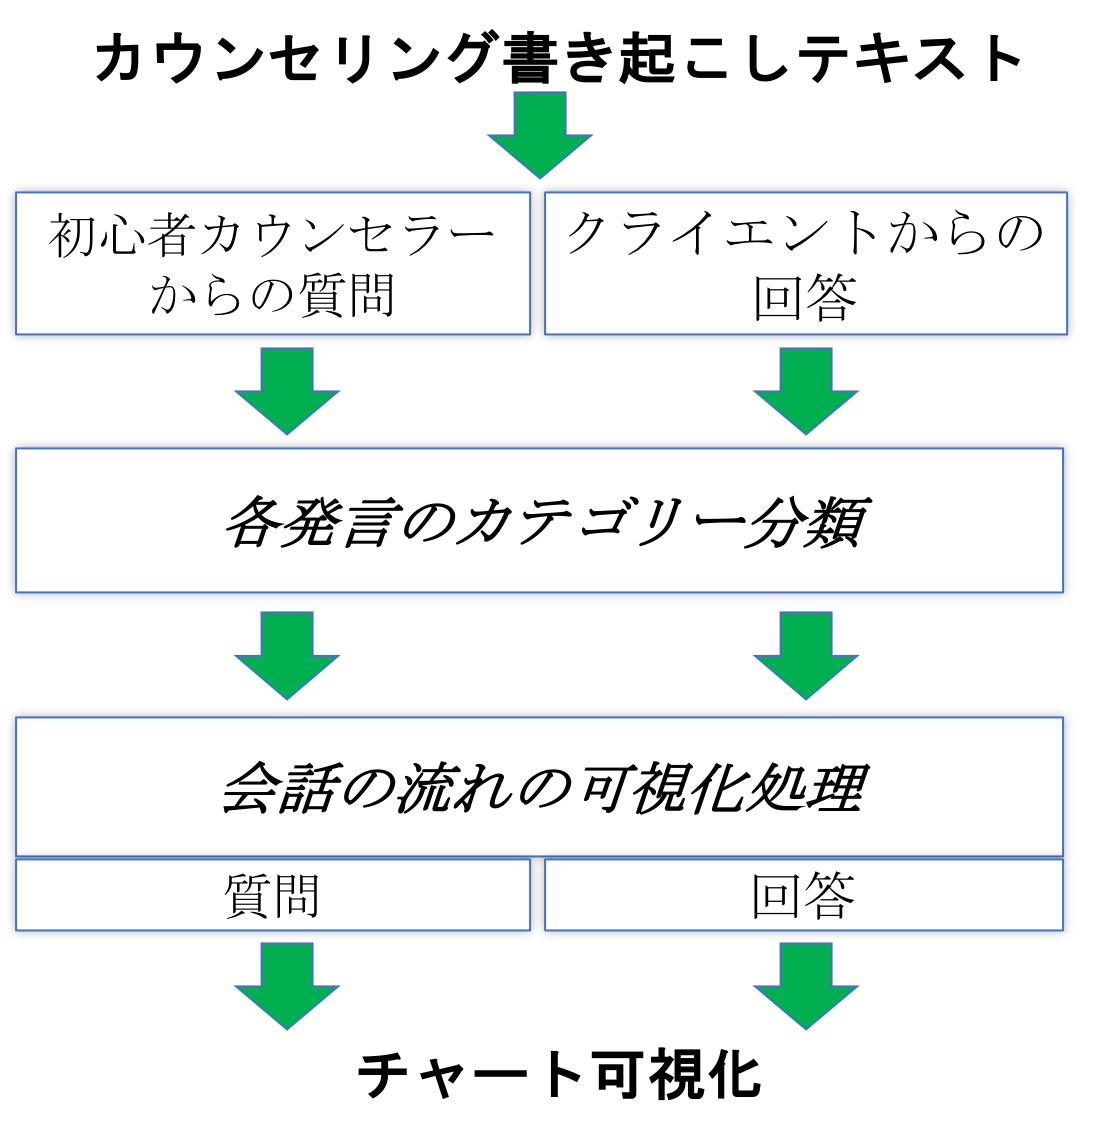
\includegraphics[width=\linewidth]{4_2.png}
  \end{center}
  \caption{提案システムの構成}
  \label{fig:4_2}
\end{figure}

\begin{figure}
  \begin{center}
    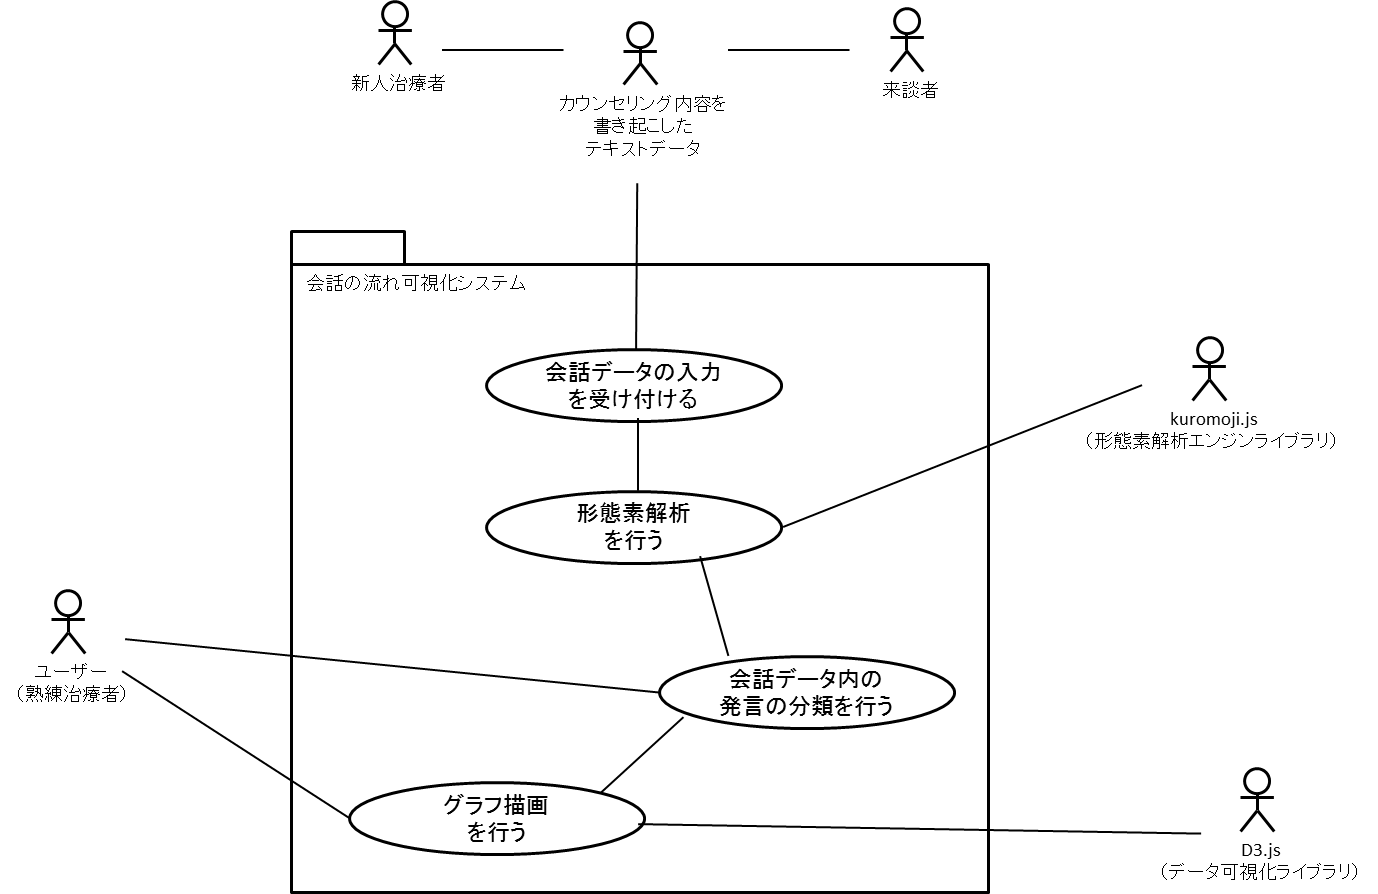
\includegraphics[width=\linewidth]{use_case_diagram.png}
  \end{center}
  \caption{提案システムのユースケース図}
  \label{fig:use_case_diagram}
\end{figure}


まず,グラフ描画前のテキストデータ処理について述べる.アクティビティ図を図
\ref{fig:activity}
に示す.アクティビティ図とはフローチャートに似た図で,いわゆるビジネスロジックにおける手続き的な流れやプログラムの制御フローを表すUMLの図である.
\begin{figure}
  \begin{center}
    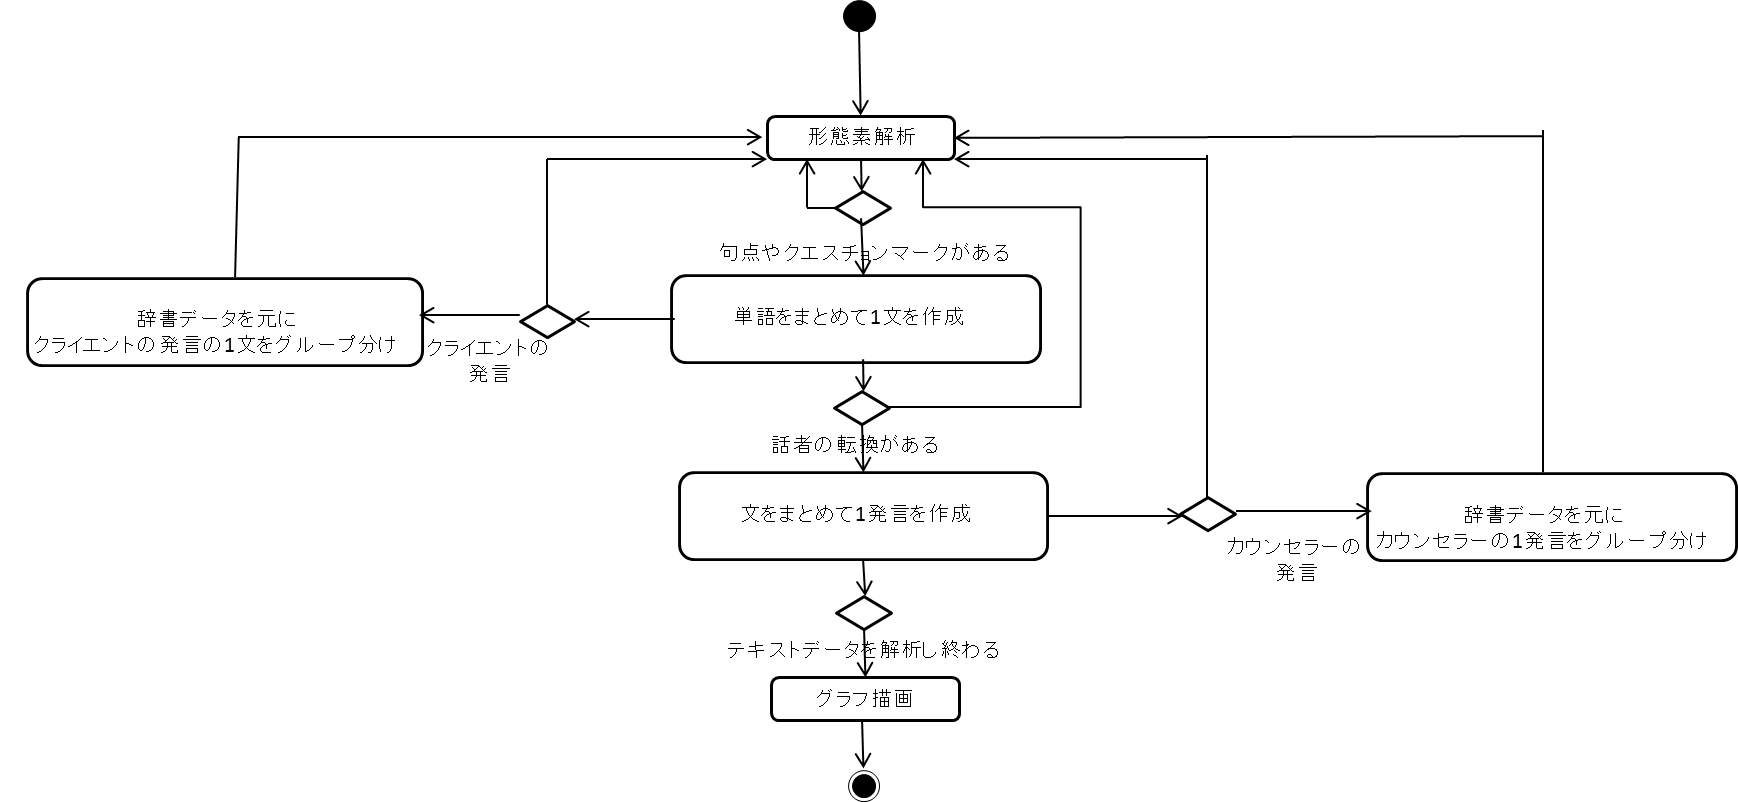
\includegraphics[width=\linewidth]{activity.png}
  \end{center}
  \caption{テキストデータ処理のアクティビティ図}
  \label{fig:activity}
\end{figure}


初めに,ブラウザ上で各テキストの会話データを読み込んで,テキストを単語ごとに区切る形態素解析を行う.会話データ読み込み前の本提案システムスクリーンショットを図
\ref{fig:yomikomimae2}
に示す.
\begin{figure}
  \begin{center}
    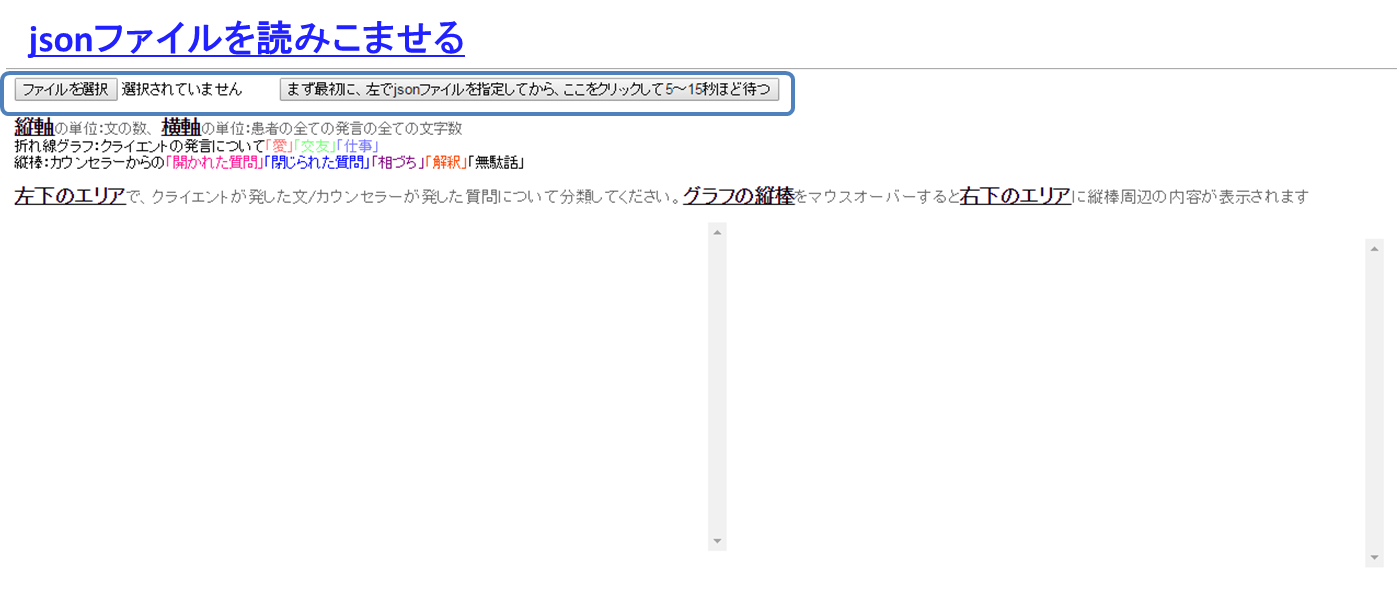
\includegraphics[width=\linewidth]{yomikomimae2.png}
  \end{center}
  \caption{会話データ読み込み前のシステムスクリーンショット}
  \label{fig:yomikomimae2}
\end{figure}
形態素解析サブシステムには,JavaScript言語の形態素解析ライブラリであるkuromoji.js\cite{kuromojijs}を使用した.kuromoji.jsは,Javaで実装されたオープンソースの日本語形態素解析エンジンKuromoji
\cite{kuromoji}
を,JavaScriptに移植したものである.

\subsubsection{1文や1発言の作成と分類}%%%%%%%%%%%%%%%%%%%%%%%%%%%%%%%%%%%%%%%
形態素解析された単語群から,句点やクエスチョンマークを終点と定義して1文ずつのテーブルをつくる.さらに,話者の切り替わりを全角コロンで定義し,全角コロンと全角コロンの間の文のグループを1発言と定義し,発言単位でテーブルをつくる.「クライエントの発言においてこれを含む文はこのグループに属するだろう」という単語を,「愛」「仕事」「交友」「自己」「スピリチュアル」ごとに指定しておき,発言データの文を構成する単語が指定された単語と一致する場合,この情報を図
%\ref{fig:4_2}
の発言データ分類サブシステムに引き渡し,発言データ分類の初期設定値を計算する.
%この初期選択において,今回は簡単化のため,複数のグループの可能性をもつ1文に対しては,「愛」の可能性があれば「愛」に,それ以外は「仕事」に分類するようにした.

%%開発

前節で述べた要件抽出にもとづいて,本研究では会話の流れ可視化システムの開発を行った.本節では,会話の流れ可視化システムの,可視化する前の処理の部分について説明を行う.


臨床的観点からは,三つのカテゴリーに人間の問題を分類するために極めて有効であると考えられる.上記分類手法から,本研究では次項で提案されたシステム,設計および実装するための要件を説明する.

このセクションでは,提案システムの設計と実装について説明する.図3は,カウンセリングでの会話の流れの可視化システムの処理手順を示している.会話の流れの可視化は)1つのカウンセリングセッションでの会話の内容を示している.このシステムでは,可視化の前処理として,カウンセリングにおける会話のテキストデータのカテゴリ分類が実行される.

まず,提案システムは,ブラウザ上で各テキストの会話データを読み,言葉にテキストを分離するために形態素解析を行う.形態素解析サブシステム内で使用されたJavaScript言語の形態素解析ライブラリであるkuromoji.js [13]は,JavaソースのKuromoji [14]からJavaScriptに移植されたオープンソース日本語形態素解析エンジンである.

次に,これらの文章は,このシステムに登録カテゴリーと文の各単語に対応するキーワードとのマッチングにより,各カテゴリに分類されている.しかし,このカテゴリの分類手法ではカウンセラーとクライエントによって各発話のテキストデータに適用し,分類結果の精度は,システムに登録されている単語辞書に依存し,分類のための正解率は非常に低いである.そのため,専門家のカウンセラーは,現在のシステムでは,最初の分類結果を確認し,手動で誤った分類結果を修正する必要があり,作業負担が大きい.クライエントのそれとは違って,私はセラピストの発話の分類は,文単位が,話し手ターン単位での分類ではないというコメントを得た.

従って,このシステムでは,担当者やカウンセラーからの1つのコメントは話者の変更によって判断される.すなわち,話者が離し始めてから別の話者話し始めるまでを1発言とし,カテゴライズする1単位とした.

このシステムでは,クライエントの発話は,それぞれの文は,アドラー心理学に基づいて,タスクエリアを分類した.図4は,表.2のようにカウンセラーの質問の自動分類手法の流れを示し,表2に示すように,他の手で,初心者のカウンセラーによって発声は5つのカテゴリに分類されている.まずはじめに,「いつ」「どこ」「何」などの5W1Hを示す疑問詞を含む発言を「開かれた質問」に分類する.次に,残りの発言から単語数が5個以下のものを「相槌」に分類する.さらに残りの発言で終助詞「か」を含む発言を「閉じられた質問」に分類する.これまでの3パターンに分類されなかったものは「解釈」か「世間話」に分類されるが,
終助詞の「ね」を含むものを「解釈」,含まないものを「世間話」とした.


%%%%%%%%%%%%%%%%%
\subsection{クライエントの回答の分類に関する要件抽出と実装}



クライエントの回答に関する分類に関しては,1発言単位ではなく1文単位で「愛」「交友」「仕事」「自己」「スピリチュアル」に分類するように変更することが求められる.

たとえば,「うちの夫は仕事にいくのを嫌がって,毎朝起きてこないんです.
それを見ているだけで腹が立つんです.自分の同僚が同じように仕事に行きたいですが
朝起きなかったという話を聞いても,さほど腹は立ちませんが,夫がそ
うなるのは絶対に許せない」という文章について,熟練したカウンセラーは次の通りに分類する.第1文は愛のタスク,第2文は仕事のタスク,第3文は愛のタスクに分類する.回答カテゴリー一覧を表\ref{table:ansCate}に記す.

\begin{table}
  \caption{回答カテゴリー一覧}
  \label{table:ansCate}
  \begin{center}
    %\includegraphics[width=\linewidth]{table2.png}
    \begin{tabular}{|l|p{7cm}|} \hline
      愛 & クライエント自身の家族や恋人との関係.家族自身の仕事関係なども含む.
      \\ \hline
      交友  & クライエント自身の友人関係.友人自身の仕事関係なども含む
      \\ \hline
      仕事 & クライエント自身の勉強・仕事の結果,上司・同僚・部下・取引先・客などとの仕事上の対人関係
      \\ \hline
      自己  &  クライエント自身との付き合い・自己存在。セルフタスク・症状などに関すること
      \\ \hline
      スピリチュアル & 超越的存在との付き合い
      \\ \hline
    \end{tabular}
  \end{center}
\end{table}

% \item 仕事のタスク(work task):クライエント自身の勉強・仕事の結果,上司・同僚・部下・取引先・客などとの仕事上の対人関係
% \item 交友のタスク(friendship task):クライエント自身の友人関係.友人自身の仕事関係なども含む
% \item 愛のタスク(love task):クライエント自身の家族や恋人との関係.家族自身の仕事関係なども含む.
% \item 自分自身のタスク(self task):自分自身との付き合い・自己存在
% \item スピリチュアリティのタスク(spiritual task):超越的存在との付き合い\cite{大友秀治2013全人的人間理解を促進するスピリチュアリティ概念に関する一考察}


原文から,カウンセラーからクライエントへの質問事項の分類の指標として,クライエントの回答をうながしてクライエント自身も気づいていなかったことを認知させるのが大事であるので,それぞれの発言量の可視化の実装を盛り込むべきであるというコメントを得た.
% ここから得られる要件は,クライエントの回答の分量に応じて,それをはさむカウンセラーの質問の縦棒をグラフ上で変えることであると考えた.

クライエントの質問に関する分類に関しては,1発言単位ではなく1文単位で「愛」「交友」「仕事」を分類するように変更することが求められる.
% たとえば,「うちの夫は仕事にいくのを嫌がって,毎朝起きてこないんである.
% それを見ているだけで腹が立つんである.自分の同僚が同じように仕事に行きたが
% らなくて朝起きなかったという話を聞いても,さほど腹は立ちないが,夫がそ
% うなるのは絶対に許せない」という文章について,専門家は次の通りに分類する.第1文は愛のタスク,第2文は仕事のタスク,第3文は愛のタスクに分類する.

% 原文から,カウンセラーからクライエントへの質問事項の分類の指標として,クライエントの質問をうながしてクライエント自身も気づいていなかったことを認知させるのが大事であるので,それぞれの発言量の可視化の実装を盛り込むべきであるというコメントを得た.ここから得られる要件は,クライエントの質問の分量に応じて,それをはさむカウンセラーの発言の縦棒をグラフ上で変えることであると考えた.

したがって,クライエントの質問に関する分類を行うために次の操作を行った。まず形態素解析された単語群から,句点やクエスチョンマークを終点と定義して1文ずつのテーブルをつくる.さらに,話者の切り替わりを全角コロンで定義し,全角コロンと全角コロンの間の文のグループを1発言と定義し,発言単位でテーブルをつくる.「来談者の発言においてこれを含む文はこのグループに属するだろう」という単語を,「愛」「仕事」「交友」ごとに指定しておき,発言データの文を構成する単語が指定された単語と一致する場合,この情報を図\ref{fig:4_2}の発言データ分類サブシステムに引き渡し,発言データ分類の初期設定値を計算する.

林田ら\cite{hayashidaJp} \cite{hayashidaEn}の手法では愛交友仕事を高確率で自動分類できたが,自己・スピリチュアルを入れないといけないので,使えなくなった.

\subsubsection{カウンセラーの質問の分類に関する要件抽出と実装}



カウンセラーの質問について,
\begin{itemize}
  \item 「開かれた質問(Open-ended Question)」
  \item 「閉じられた質問(Closed-ended Question)」

\end{itemize}
だけでなく,
\begin{itemize}
  \item 「解釈や助言」
  \item 「相槌」
  \item 「世間話」
\end{itemize}

という分類を追加してほしいというコメントを得た.以上の詳細を表\ref{table:queCate}にまとめる.
\begin{table}
  \caption{質問カテゴリー一覧}
  \label{table:queCate}
  \begin{center}
    %\includegraphics[width=\linewidth]{table2.png}
    \begin{tabular}{|l|p{7cm}|} \hline
      開かれた質問 & 5W1H(「何処で」「誰と」「なぜ」等)で問うことで,クライエントが自ら回答内容を
      考えていくための情報収集を目的とした質問
      \\ \hline
      閉じられた質問  & 「昨日母と話しましたか?」等,Yes/Noで答えさせる質問
      \\ \hline
      相槌 & 「はい」「そうですね」等
      \\ \hline
      解釈と助言  &  カウンセラーの考えである解釈の投与,および助言\\ \hline
      世間話 & 上記以外の,カウンセラーの発話内容に直接は結びつかないもの \\ \hline
    \end{tabular}
  \end{center}
\end{table}

% \begin{table}[htb]
%   \begin{tabular}{lcrr}
%     メニュー & サイズ & 値段 & カロリー \\
%     牛丼 & 並盛 & 500円 & 600 kcal \\
%     牛丼 & 大盛 & 1,000円 & 800 kcal \\
%     牛丼 & 特盛 & 1,500円 & 1,000 kcal \\
%     牛皿 & 並盛 & 300円 & 250 kcal \\
%     牛皿 & 大盛 & 700円 & 300 kcal \\
%     牛皿 & 特盛 & 1,000円 & 350 kcal
%   \end{tabular}
% \end{table}

またクライエントの回答に関する分類とは異なり,カウンセラーの質問に関する分類は1文単位ではなく1発言単位での分類でよいというコメントを得た.

カウンセラーの発言の分類について,まずカウンセラーの発言も,次章で述べる初期分類は適当ではないことがあるので,クライエントからの返答だけでなく,カウンセラーの質問区分けも手動で修正したいというコメントを得た.

以上のコメントにしたがい、実装を行う。カウンセラーの1発言についても,クライエントの発言の1文ごとの分類と同様に,関連する単語をあらかじめ指定しておき,必要情報を
\ref{fig:4_2}
の発言データ分類サブシステムに引き渡し,発言データ分類の初期設定値を計算する.

ここで会話データを入力した後のカウンセラーの初期分類状態の分類手法について説明する.今回の実際の会話データ15個のうち,カウンセラーの発言数は398発言あったが,本システム要件の質問分類の「相槌」に含まれるべき短文に「そうであるか」というフレーズが41箇所あった.富士通株式会社は質問文判定について特許
\cite{tokkyo}
を取得しているが,富士通株式会社の特許技術において行われている「(る)か」という文の終わり方だけで質問判定を行うだけでは,「そうであるか」というフレーズも自動的に「相槌」ではなく「閉じられた質問(Closed-ended Question)」に分類してしまうので不適当である.



% また,質問内容は,前章の要件通り5種類に分類され,後述する縦棒アイコンの色の割り当ては次の通りである.赤色は5W1H「いつ」「どこで」「誰が」「何を」「どのように」「どうした」などで問われるような「開かれた質問(Open-ended Question)」,青色はYes/Noで答えられる,あるいは一言だけで簡単答えられるような「閉じられた質問(Closed-ended Question)」,紫は「相槌」,オレンジはクライエントの問題をカウンセラーがどう「解釈」しているかの確認,黒は「世間話」を表現している.第1章で述べた通り,クライエントが何に問題意識を感じているかに対してカウンセリングでカウンセラーの関心を傾聴するには,カウンセラーは「閉じられた質問(Closed-ended Question)」よりも「開かれた質問(Open-ended Question)」をしたほうがよいとされている

% まず会話データ入力サブシステムでカウンセリングの書き起こしテキストデータを入力し,形態素解析サブシステムに引き渡す.
% 形態素解析サブシステムでは,カウンセラーの1発言についても,クライエントの発言の分類と同様に,関連する単語をあらかじめ指定しておき,必要情報をFig.1の発言データ分類サブシステムに引き渡し,発言データ分類の初期設定値を計算する.

本システムにおける,会話データを入力した後のカウンセラーの初期分類状態の分類手法を簡単に図
\ref{fig:5_2}
に示す.
\begin{figure}
  \begin{center}
    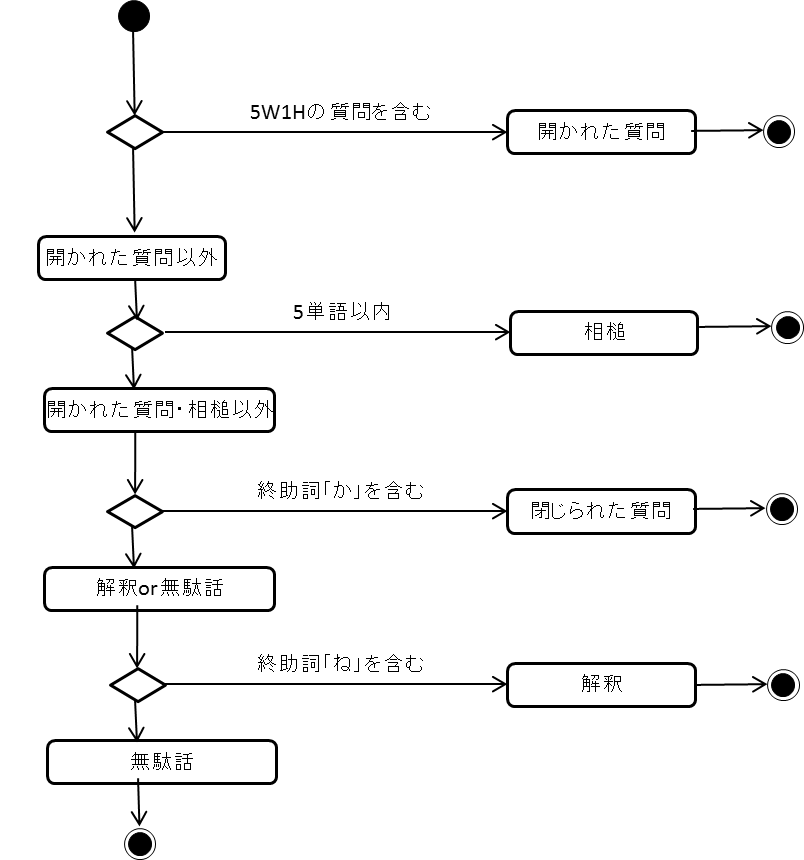
\includegraphics[width=\linewidth]{5_2.png}
  \end{center}
  \caption{カウンセラーの質問の初期分類手法}
  \label{fig:5_2}
\end{figure}
まず「いつ」「どこ」「何」などのいわゆる5W1Hを示す疑問詞をもつ発言を「開かれた質問(Open-ended Question)」に分類する.次に残りの発言のうち,単語数が5個以下のものを「相槌」に分類する.さらに残りの発言のうち終助詞「か」を含む発言を「閉じられた質問(Closed-ended Question)」に分類する.今までの3つに分類されなかったものは「解釈」か「世間話」に分類されるわけだが,終助詞の「ね」を含むものを「解釈」,含まないものを「世間話」とした.



% 一方,クライエントの発言の各1文の分類手法として,ヨーガセラピーが基本としているアドラー心理学の3つのライフタスク7)(「愛」「仕事」「交友」)分類カテゴリとして用いることにした.
次に,会話データを発言データ可視化サブシステムに受け渡し,カウンセラーからの質問の分類結果と,クライエントの発言のカテゴリ分類結果を併せて,時間経過に沿った分布変化としてグラフによる可視化表示を行う.


% システム設計と実装








%\subsection{クライエントの回答に関する分類} %%%%%%%%%%%%%%%%%%%%%%%%%%




%\subsection{カウンセラーの質問に関する分類} %%%%%%%%%%%%%%%%%%%%%%%%

\section{可視化結果}

前節では,会話の流れ可視化システムの可視化前の処理の部分の実装について説明を行った.本節では,その前処理後の可視化の処理の部分について説明を行う.


%%可視化結果をゴリゴリ説明


%のスライダーを動かすことによって,本研究ではどのような文を時系列に沿ってどのような文に,例えば,人間関係からチャートを表示した.また,図2に示すように,それが可能な,対応する動詞の文章を表示することによって,本研究では,矢印は,図手段として,元のどのテキストを知ることができる.

本研究では,可視化のためにD3.js\cite{vand3}を用いた.D3.jsはウェブブラウザ上で動的なコンテンツを可視化するためのJavaScriptのライブラリであり,ニューヨーク・タイムズ紙サイト内のグラフ描画などに用いられている.




\subsection{グラフ描画}
以上がグラフ描画前のテキストデータ処理である.その後,カウンセラーからの質問形態と, 「愛」「仕事」「交友」「自己」「スピリチュアル」の文のグループの時間経過に沿った分布変化を可視化する.グラフ描画の際に,会話データを発言データ可視化サブシステムに受け渡す.このサブシステムでは,データ可視化ライブラリD3.js
\cite{bostock2012d3}
を使用した.模擬会話データを入力し、後述する積み重ね折れ線グラフを出力した際の結果を図
\ref{fig:6_1}
に示す.
% また模擬会話データの原文と,模擬会話データ時の初期自動分類結果を表
% \ref{table:book1}
% に示す.
\begin{figure}
  \begin{center}
    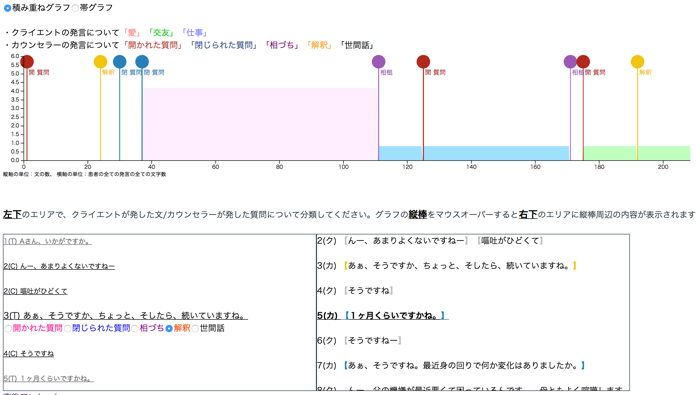
\includegraphics[width=\linewidth]{6_1.png}
  \end{center}
  \caption{模擬会話データでのシステム出力結果(積み重ね折れ線グラフ)}
  \label{fig:6_1}
\end{figure}

% \begin{table}
%   \caption{模擬会話データでの初期表示用自動分類結果}
%   \label{table:book1}
%   \begin{center}
%     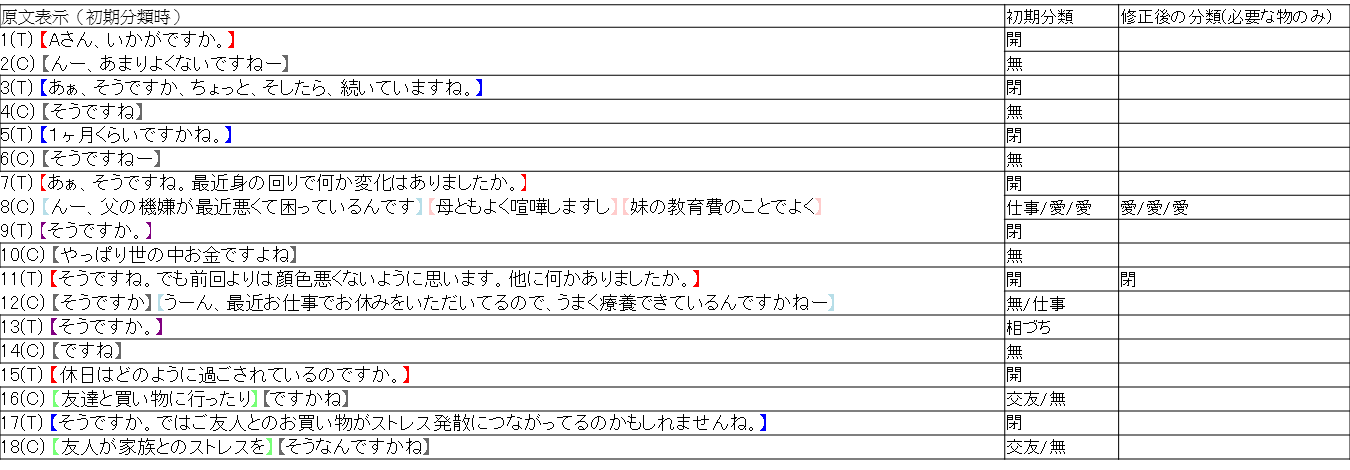
\includegraphics[width=\linewidth]{book1.png}
%   \end{center}
% \end{table}


\subsubsection{積み重ね折れ線と縦棒のグラフ}
次に,クライエント発言ビューについて説明する.
図
\ref{fig:6_1}
において,まず積み重ね折れ線グラフはクライエントの1回の発言の中での,アドラー心理学の各カテゴリの分布を可視化している.ただし1回の発言は,話者の交代を発言の区切れ目とする.この積み重ね折れ線グラフにおいて薄い水色は「仕事関係」,ピンク色は「愛(恋愛・愛関係)」,薄い緑色は「交友(友人関係)」、黄色は「自己」、紫は「スピリチュアル」に密接に関係する単語を含む文の分布を表している.

横軸は時間軸を表現している.ただし対象データである書き起こしテキストデータからは実際の経過秒数は読み取れないので,読み込ませたデータ内におけるクライエントの発言量の累計の文字数を横軸,つまり時間軸とした.後述するカウンセラーの質問を表現する縦棒はこの時間軸にそって出現する.
% カウンセラーとクライエントの発言の入れ替わりがわかりやすいように,積み重ね折れ線グラフがクライエントの発言のグループ分布をちょうど表しているのは便宜上発言部分の中央部分になっている.

縦軸は発言中の1文の数のうち,どのグループに何文入っているかという文の数を表している.

%ここで会話データを入力した後のクライエントの発言の各1文の初期分類状態の分類手法について説明する.
%まず,あらかじめこちらで
%次に,各単語群を含むクライエントの発言の1文をグループ分けをしていった.


Ericら\cite{taskdriven}は,トピックモデリングによって分けたトピックの時間分布を上下の非対称積み重ね折れ線グラフによって可視化した.一方本研究では,カウンセラーとクライエントの会話において,クライエントは文ごとに,カウンセラーは発言ごとに描画を行いたい,かつ選択肢表示のためにグラフを省スペースしたいという観点から,カウンセラーの発言を横軸より下に折れ線グラフとして描画するのではなく,クライエントの発言のグループ分布を示す積み重ね折れ線グラフに重ねて縦棒として表示するようにした.こうすることによって,クライエントとカウンセラーの発言が交互に描画されるので,クライエントとカウンセラーの発言の関連性がわかりやすくなった.積み重ね折れ線グラフに重なっている縦棒は,カウンセラーの質問内容の形態を示す.縦棒の色分けは、赤が「開かれた質問」、青が「閉じられた質問」、オレンジが「解釈や助言」、紫は「相槌」、黒が「世間話」を表す。




\subsubsection{帯グラフ}

さらに,もう一つの可視化方法として帯グラフによる結果を図\ref{fig:obi}に示す.図\ref{fig:6_1}の積み重ねグラフ同様,横軸は時間軸を表す.2本の帯グラフのうち,上側はカウンセラーの発言,下側はクライエントの発言を表す.初心者のカウンセラーの質問とクライエントの回答の各分類カテゴリ及び色分けについては,それぞれ積み重ね折れ線グラフにおける積み重ね折れ線と縦棒の場合と同様である.

積み重ね折れ線グラフはカウンセラーの発言を縦棒のみで表示しているのに対し,帯グラフはクライエントの発言だけでなくカウンセラーの発言も文量情報を持った表示をしている.そのため、初心者のカウンセラーの質問とクライエントの回答の帯グラフの各色分けされた区間内の長さは、それぞれの発言の長さを表している。対象データである書き起こしテキストデータからは実際の経過秒数は読み取れないので,読み込ませたデータ内における初心者のカウンセラーとクライエント2人の発言量の累計の文字数を横軸とした。

\begin{figure}
  \begin{center}
    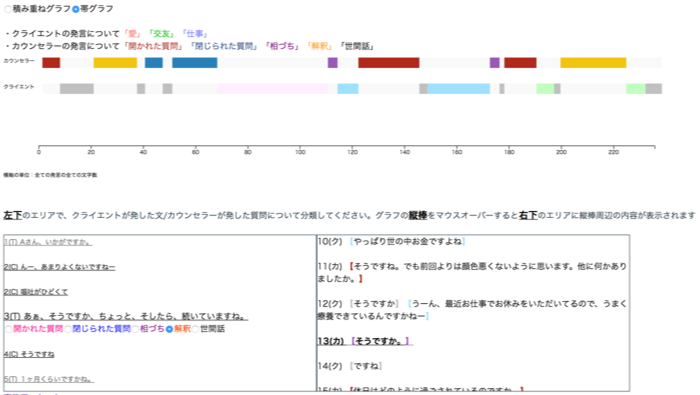
\includegraphics[width=\linewidth]{obi.png}
  \end{center}
  \caption{模擬会話データでのシステム出力結果(帯グラフ)}
  \label{fig:obi}
\end{figure}

\subsection{発言分類手動修正機能}
積み重ね折れ線グラフが描画された後に,グラフ左下のラジオボタンエリアにて,クライエントの発言の各1文およびカウンセラーの各1発言において,分類を変えると即時にグラフ描画に変更が適用されるようにした.この手動変更した結果は、localStorageを用いてユーザーの使った各ブラウザ上に保存され、CSV出力/入力によって他ユーザーに引き継ぎ可能である。
%本ラジオボタンエリアがみたした要件については,付録にて記述する.

%\section{要件抽出}

\subsection{原文表示機能}
どこがどの発言を表しているかわからないという問題に対しては,両グラフのそれぞれ初心者のカウンセラーの質問やクライエントの回答を表す箇所にマウスカーソルをあわせることによって,グラフ右下に周辺の発言を表示する機能を追加することで解決を図った.見やすさのため,グラフの色に対応した文字色ではなく黒い文字で各発言を表示し,それをグラフと対応した色の隅付き括弧【】で囲うようにした.


%\section{開発}

%%修論からパクってくる


%
% \subsection{ケーススタディ}
%
% 前節までで,本システムの前処理手順および可視化手法と可視化結果について述べた.本節では本システムにもとづいたユースケースについて述べる.

\section{ユーザー評価実験と考察}

前節までは,会話の流れ可視化システムの開発およびケーススタディについて説明を行った.本節では,会話の流れ可視化システムを用いて「」という仮説を検証するために行ったユーザ評価の目的・手法・結果・考察についてのべる.% カウンセラー習熟度評価支援システムは,主に,
%
% %%ユーザエバリュエーションをゴリゴリ説明
%
%
%
%
% 専門カウンセラーが,彼は「私はBが私の意志に従うことをしたい」という考えが消えていることが分かったと述べた.
%
% 自己閉じタスクが増加した.認知の補正の進行は,することができた 量変更することによって確認 矢印の(複数カウンセリングの全体図)をし,元のテキスト表示で品質を確認. 本研究では,我々の提案文字チャートの可視化は,カウンセラーは見つけることができることを検討してください のいくつかの種類がことを ,クライエントの 認知の修正作られた.

\subsection{シグマ値法}
多数の意見項目などを多変量解析で分析する際に,態度を測るものさしであるカテゴリー尺度は,本来は順序尺度なので,間隔尺度に換算して重み付ける必要がある.しかし通常は,回答カテゴリーのコード番号を間隔尺度の得点として簡便に用いている.

通常の例の場合に対して,心理学では,カテゴリーの順序尺度を間隔尺度に換算する手法を持っている.その一つにシグマ値法(系列カテゴリー法ともいう)が存在し\cite{likert1932technique},現在でも様々な研究分野におけるカテゴリー得点の換算に用いられている\cite{シグマ値法使ってる} \cite{岩本隆2016人事}.シグマ値法は,意見項目の各カテゴリーに対する一連の回答率を,標準正規分布の面積と考え,面積に対応する縦座標と面積の比という間隔尺度に置き換える手法である.

標準正規分布は,元のデータを0,標準偏差1.0に換算したデータのことである.シグマ値法においては,回答カテゴリーの回答率を標準正規分布の面積と考えて,面積に対応する縦座標の比に置き換えることによって,順序尺度を間隔尺度に置き換えることが出来ている.

シグマ値法は以下の手順に従って算出される.
\begin{enumerate}
  \item 各カテゴリーの順番を下位のものから上位のものに整列させる
  \item 各カテゴリーへの度数から比率を計算する
  \item 各カテゴリーの累積の比率を算出して,下限値から上限値までを計算する.
  \item 各カテゴリーの累積の比率の最小値と最大値を標準正規分布の縦座標に置き換える
  \item シグマ値を計算する
  \item カテゴリー得点の計算を行う.
\end{enumerate}

以上のシグマ値法で換算した値を用いて,多変量解析をおこなうことによって,「悪いが1点,やや悪いが2点,……」のようなカテゴリー得点をカテゴリーの数字で代替する通例の手法よりも明快な解析結果が得られると言われている.

ガウスの誤差関数
\begin{equation}
  erf(x) = \frac{2}{\sqrt{\pi}}\int_0^x e^{-t^2} dt
\end{equation}
を用いると,標準正規分布の累積分布関数F(x)は
\begin{equation}
  F(x) = \frac{1}{2}(1+erf\frac{x}{\sqrt{2}})
\end{equation}
で表される.この逆関数\begin{equation}F^{-1}(x)\end{equation}を用いて,標準正規曲線の面積に対応する標準得点Z(p)は

%Z(p)=-F-1(1-p)

\begin{equation}
  Z(p) = -F^{-1}(1-p)
\end{equation}

でである.標準得点Zに対応する縦座標yは,標準正規曲線の確率密度を求める式によって表され,
\begin{equation}
  y(Z)=\frac{1}{\sqrt{2\pi}}exp(-\frac{Z^2}{2})
\end{equation}
となる.






\subsection{可視化手法の比較に関する評価と考察}
上辻\cite{uetsuji}が取り扱った積み重ね折れ線チャートの形状との比較を行った.前節で述べた会話の流れの可視化システムを,3名の熟練したカウンセラーに評価者として実際に使用してもらうことで,システム評価を行った.
熟練したカウンセラーの平均年齢は55歳,平均臨床歴は29年であった.

本項で述べる比較評価の目的は、「初心者のカウンセラーの関心がクライエントの関心にどのくらい傾聴されているか」が、上辻\cite{uetsuji}が取り扱った積み重ね折れ線チャートでの評価よりも、本グラフの帯グラフ可視化モードの方がわかりやすい、という仮説の検証である。まず評価者は,積み重ねグラフ,帯グラフそれぞれについて,あらかじめ表示されている可視化結果に対して,時系列に沿ってマウスカーソルを合わせることで,カウンセリングの流れを一通り確認する.

\subsubsection{6段階評価のアンケート}


その後,6段階評価によるアンケート質問に回答を行う.6段階評価のアンケートの質問項目,および各質問に対する選択肢とその配点を表\ref{table:keijouAnketo}に示す.表\ref{table:keijouAnketo}の各質問項目は,積み重ねグラフ,帯グラフそれぞれに対して行った.積み重ねグラフ,帯グラフについて,各質問項目に対する6段階評価の平均値の結果を図\ref{fig:keijouAnketo}に示す.図\ref{fig:keijouAnketo}の結果より,全ての項目において,積み重ねグラフより帯グラフの方が優れていることがわかった.

\begin{table}
  \caption{Three life task based on Adler psychology.}
  \label{table:keijouAnketo}
  \begin{center}
    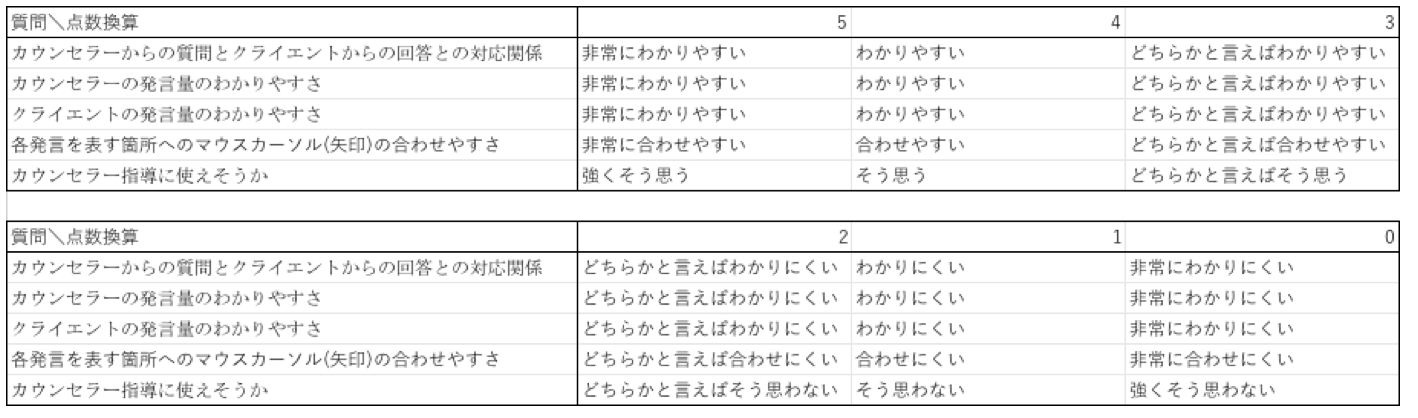
\includegraphics[width=\linewidth]{point.png}
    % \begin{tabular}{|l|p{7cm}|} \hline
    % Work task & Impermanent human relationship \\ \hline
    % Friendship task  & Permanent, and do not fate together human relationship \\ \hline
    % Love or Family task & Fate together human relationship \\ \hline
  % \end{tabular}
\end{center}
\end{table}

\begin{figure}
  \begin{center}
    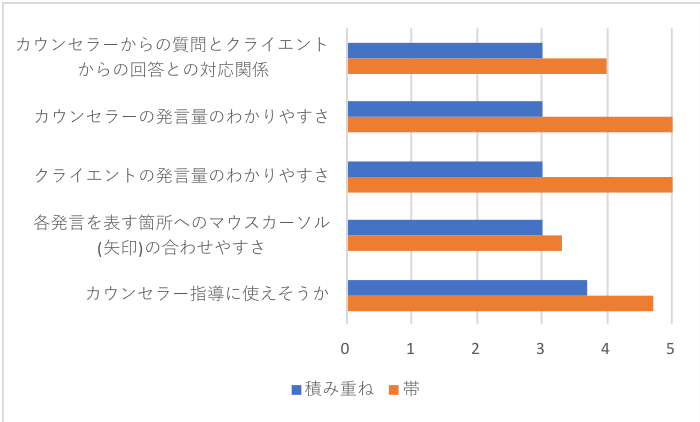
\includegraphics[width=\linewidth]{keijouAnketo.png}
  \end{center}
  \caption{形状比較実験の6段階評価の平均値}
  \label{fig:keijouAnketo}
\end{figure}

%%有意差,相関関係

\subsubsection{自由記述のアンケート}

さらに本評価では,以下の1.〜5.に記す自由記述の質問を行った.

\begin{enumerate}
  \item 帯グラフを見て,初心者のカウンセラーに対してどのような指導ができるでしょうか
  \item グラフについて,その他全体的に何かご意見があれば,ご回答ください
  \item このシステム全体を用いて,初心者のカウンセラーに対して指導できそうなことがあれば,ご回答ください
  \item 原文表示機能について何かご意見があれば,ご回答ください
  \item このシステムについて,何か他に欲しい機能があれば,ご回答ください
\end{enumerate}

1つ目の質問に対しては,
\begin{itemize}

  \item 一回のカウンセリング全体を俯瞰し大まかなカウンセリングの流れを指導
  \item クライエントとカウンセラーが時系列で対比しながら見ることができるので,一回の面接での流れ,例えば,前半はクライエントに多く喋ってもらっていたのが,後半ではカウンセラーが喋っていたとか,解釈の時に発言量が多いとかが指導できるように思った
\end{itemize}
といった回答が得られた.これより,全体を俯瞰して発言量の分布の変化を基に初心者のカウンセラーに対して,様々な指摘を行えることが考えられる.
質問2.に対しては「帯グラフで,それぞれの発言内容の語数や時間が表示されれば,さらに便利かなと思った」という回答が得られた.
質問3.に対しては

\begin{itemize}

  \item カウンセラーの発言のチェックとクライエントの関心に関心を向けているかのチェック」「一回のカウンセリングでカウンセラーとクライエントがどのような作業を協力して行っているのか理解を深めること,カウンセリングが成立するためにはカウンセラーとクライエントの間で相談的人間関係が構築できていることが前提となることを理解するのに役立つ
  \item カウンセリングがこのように可視化されることだけでも,とても有意義だ
  \item この結果をもとに,カウンセリングを再構築するための材料としても使える
\end{itemize}
といった回答が得られた.
質問4.に対しては「カウンセラー,クライエントがどこでどんな発言をしているのか確認するのに役に立つと思った」という回答が得られた.
以上の結果から,積み重ねグラフよりも帯グラフの方が,初心者のカウンセラー指導に優れていると結論づけられる.また全体として,本システムが初心者のカウンセラーに対する指導を行うために,会話の流れが適切に可視化されていることが,複数名の熟練したカウンセラーからの回答によって結論づけられると考える.
質問5.に対しては

\begin{itemize}

  \item カウンセラー,クライエントの発言を音声で確認できる機能,カウンセリング中のクライエントの身体の動きの変化(カウンセリング開始から本題にはいるまで〈相談的人間関係構築がなされているかどうか確認のため〉また特にカウンセラーが解釈投与した直後のクライエントの身体の動き〈解釈投与に対してクライエントがどのような認識反射をおこなっているのかを確認するため〉)についても記されていると便利だと思う
  \item 複数の内容が入った文について,うまく分類できればもっと便利
  \item 内容分類項目のアレンジ機能(追加,修正)
\end{itemize}
といった回答が得られた.
以上の回答から,本システムのユーザービリティの改善や機能追加についてさらなる検討を行う必要があり,今後の課題とされる.



\subsection{カウンセラーによる本システムの有用性に関する評価と考察}%%%%%%%%%%%%%%%%%%%%%%%%%%%%%%%%%%%%%%%%%%%%%%%%%%%%%%%%%%%%%%%

%%コメントでゴリゴリ稼げる

前項では,上辻ら\cite{uetsuji}が2016年に発表した積み重ね折れ線チャートよりも,本研究で提案した本システムの帯グラフの方が,初心者のカウンセラーに対する指導を行うためにより適切な可視化手法であることが分かった.前項で述べたユーザー評価からわかったことを元に,実際のカウンセリング内容の原文を用いて,図\ref{}のような実際のカウンセラー内での事例検討会に近いスタイルフォーマットの原文のみを読んでの初心者のカウンセラー指導と,本研究で提案した帯グラフを用いた初心者のカウンセラー習熟度評価支援システムを用いての初心者のカウンセラー指導との比較実験について,本項にて述べる.

本項で述べる比較評価の目的は、「初心者のカウンセラーの関心がクライエントの関心にどのくらい傾聴されているか」が、今日行われている原文を読むだけでの評価よりも、本グラフの帯グラフ可視化モードの方がわかりやすい、という仮説の検証である。会話の流れの可視化システムを,5名のカウンセラーに評価者として実際に使用してもらうことで,システム評価を行った.

本研究ではスーパーヴァイザーがスーパーヴァイジーのカウンセリング内容の指導や分析を支援するために,「カウンセリングにおける会話の流れの可視化システム」を開発した.
本システムは,初心者のカウンセラーの質問とクライエントの回答の内容をそれぞれカテゴリ分類して,その結果を時間経過に沿ったカテゴリの分布変化として可視化表示した.

\begin{enumerate}

  \item 事前アンケートへのご回答
  \item 作業を始める前に
  \item 皆様に行っていただく作業
  \begin{enumerate}
    \item 作業1(原文を呼んでの評価) → 作業後アンケートのご回答
    \item 作業2(提案システムを使っての評価)→ 作業後アンケートのご回答
  \end{enumerate}
\end{enumerate}
の流れで評価を行った.まず評価者は,
\begin{enumerate}

  \item 原文
  \item 帯グラフそれぞれについて,あらかじめ表示されている可視化結果に対して,時系列に沿ってマウスカーソルを合わせる
\end{enumerate}
ことで,カウンセリングの流れを一通り確認する.




\subsubsection{6段階評価のアンケート}

その後,6段階評価によるアンケート質問に回答を行う.6段階評価のアンケートの質問項目,および各質問に対する選択肢とその配点をTable 1に示す.Table 1の各質問項目は,原文,帯グラフそれぞれに対して行った.積み重ねグラフ,帯グラフについて,各質問項目に対する6段階評価の平均値の結果を図\ref{fig:q1},\ref{fig:q2},\ref{fig:q3}に示す.



\begin{figure}
  \begin{center}
    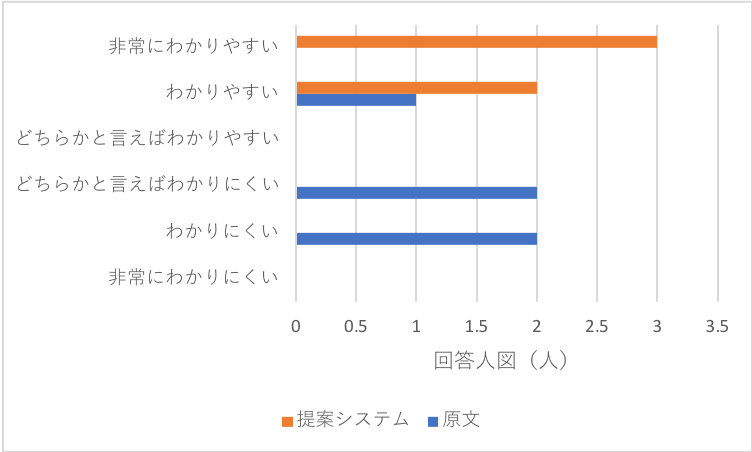
\includegraphics[width=\linewidth]{q1.png}
  \end{center}
  \caption{今回取り扱ったカウンセリングの会話データを,作業1,2の手法で閲覧することで,「初心者のカウンセラーがどの程度開かれた質問を使用しているか」が,どの程度わかりやすかったですか?}
  \label{fig:q1}
\end{figure}

\begin{figure}
  \begin{center}
    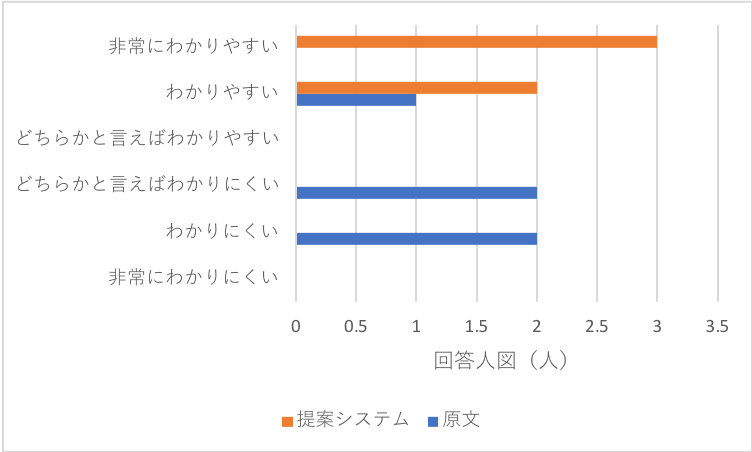
\includegraphics[width=\linewidth]{q1.png}
  \end{center}
  \caption{回取り扱ったカウンセリングデータを作業1,2の手法で閲覧することで,「カウンセラー側が自分の意見を言いたがる程度」が,どの程度わかりやすく感じたでしょうか?(図\label{fig:q1}と同一の結果となった)}
  \label{fig:q1}
\end{figure}

\begin{figure}
  \begin{center}
    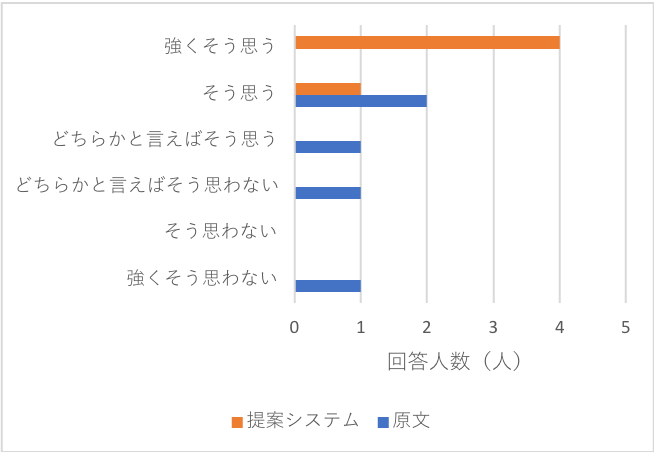
\includegraphics[width=\linewidth]{q3.png}
  \end{center}
  \caption{作業1,2の閲覧手法は初心者のカウンセラー指導に使えると,どの程度思いましたか?}
  \label{fig:q3}
\end{figure}

前前節で述べたシグマ値法を用いて,
各質問に対する回答においてシグマ値法で点数を算出した結果を表\ref{table:sigma}, \ref{table:sigma2}に示す.


\begin{table}
  \caption{質問1,2に対する回答においてシグマ値法で算出した点数}
  \label{table:sigma}
  \begin{center}
    %     \includegraphics[width=\linewidth]{table1.png}
    \begin{tabular}{|l|r|} \hline
      非常にわかりやすい & 1.159 \\ \hline
      わかりやすい  & 0.129 \\ \hline
      どちらかと言えばわかりやすい & なし \\ \hline
      どちらかと言えばわかりにくい & -0.532 \\ \hline
      わかりにくい  & -1.400 \\ \hline
      非常にわかりにくい & なし \\ \hline
    \end{tabular}
  \end{center}
\end{table}

\begin{table}
  \caption{質問3に対する回答においてシグマ値法で算出した点数}
  \label{table:sigma2}
  \begin{center}
    %     \includegraphics[width=\linewidth]{table1.png}
    \begin{tabular}{|l|r|} \hline
      強くそう思う & 0.966 \\ \hline
      そう思う  & 0.129 \\ \hline
      どちらかと言えばそう思う & -0.677 \\ \hline
      どちらかと言えばそう思わない & -1.045 \\ \hline
      そう思わない  & なし \\ \hline
      強くそう思わない & -1.755 \\ \hline
    \end{tabular}
  \end{center}
\end{table}


\begin{enumerate}

  \item 今回取り扱ったカウンセリングの会話データを,作業1,2の手法で閲覧することで,「初心者のカウンセラーがどの程度開かれた質問を使用しているか」が,どの程度わかりやすかったですか?
  \item 今回取り扱ったカウンセリングデータを作業1,2の手法で閲覧することで,「カウンセラー側が自分の意見を言いたがる程度」が,どの程度わかりやすく感じたでしょうか?
  \item 作業1,2の閲覧手法は初心者のカウンセラー指導に使えると,どの程度思いましたか?
\end{enumerate}
の質問に対する回答において,作業1(原文を読む)と作業2(提案システムを使う)に対する回答間について、
その点数を用いてt検定を行った結果,Q1,2に関してはt=0.0432,Q3に関してはt=0.0309となり、有意差が見られた。
これらの結果から,
「原文を読むだけ」より「本提案システムを用いる手法」の方が,
\begin{itemize}
  \item 「初心者のカウンセラーがどの程度開かれた質問を使用しているか」がわかりやすい
  \item 「カウンセラー側が自分の意見を言いたがる程度」がわかりやすい
  \item 初心者のカウンセラー指導に使える
\end{itemize}
という知見が得られた.


%%有意差,相関関係
\subsubsection{自由記述のアンケート}
%
%
% さらに本評価では,以下の(1)~(5)に記す自由記述の質問を行った.
%
%
%
% \begin{enumerate}
%   \item 帯グラフを見て,カウンセラーに対してどのような指導ができるでしょうか
%   \item グラフについて,その他全体的に何かご意見があれば,ご回答ください
%   \item このシステム全体を用いて,カウンセラーに対して指導できそうなことがあれば,ご回答ください
%   \item 原文表示機能について何かご意見があれば,ご回答ください
%   \item このシステムについて,何か他に欲しい機能があれば,ご回答ください
% \end{enumerate}




%%コメントでページ数稼げる

以下のようなエキスパートコメントを得た.尚,「作業1」が原文を読む作業,「作業2」が提案システムを使う作業、「CL」とはクライエントのことである.
\begin{itemize}
  \item 作業2について・・・大変ユニークなシステムで,開かれた質問量とその後のCLの語りの割合がとても見やすかったです.また,原文表示機能とのリンクが,素晴らしいと思います.このままでも,十分に利用したいと思える機能ですが,出来が良いだけに欲が出ました.以下の要望があります.部分的な事は分かりましたが,全体の流れの中で最終的にどのくらいの割合(何%)になっているのかまで分かると,更に詳細に自己分析する手助けになると思います.また,何ケースも経験を重ねていく中で,質問がうまくなると開かれた質問の%が増えて行き,それに伴いCLの語りの%が増えるような現象がみられると,なお面白い研究だと思えます.

  \item 今回の例では,理想像の母親に対しての,確認の作業を閉じられた質問で展開し,その後のCLの回答を踏まえて,解釈を提示していき,理想の母親に近づく為の考えを導いていく為に,開かれた質問が展開されてきていると感じました.その流れが,作業1よりも,作業2の方で,明確に理解出来ました.
  \item 原文だけではイメージしにくい5つの分類を明快に色分けされ色ごとに会話の長さが直線表示されたことで解釈等で結構喋っていることが分かりました.また世間話の項目もある事で,振り返りの際に積極的に無駄をなくすことにつながると思います.それらが質問で投げかける言葉の選択や,カウンセリングの質を上げる事になると思いました.

  \item 言葉数が多いということだけでも意見を言いたがっていることがわかる.説明的であり,クライエントに自分の考えを一方的に押し付けている.クライエントの発する言葉をきちんと捉え,その言葉の意味を聞いていくというのではなく,カウンセラー側の言葉を使って解釈をしている.
  \item 作業1のみより作業2の可視化がある事で自己のカウンセリングの内容が客観的に見やすい.5つの分類の量や種類(何を多用してるか,特に質問の種類)を把握出来る事で,スーパーヴァイズもしやすいと思うし,受ける側も理解しやすいと思われる.次の目標が立てやすい.また,記録を残していくことで自己成長の軌跡が残せるのではないか.ただ,作業2のみだとビジュアルに意識が散乱するので 本筋や全体を把握するのに作業1も欲しい.
  \item 色別に,どんな種類の問や,回答があるのかが,一目で理解でき,それが,脳裏に残っている.そして,色の部分と,CLやカウンセラーの話した内容を同時に,理解していく作業を一通り行っただけで,こんなに詳しく,アンケートに応えられている事が驚きです.逐語録を読むだけだと,いつもボーっとしてしまい,どんな内容か,理解出来ない私でも,瞬時に,内容が理解でき,分析出来るシステム,是非,様々な場面で使えたらと思いました.

\end{itemize}

「原文だけではイメージしにくい5つの分類を明快に色分けされ色ごとに会話の長さが直線表示されたことで解釈等で結構喋っていることが分かりました」「作業1のみより作業2の可視化がある事で自己のカウンセリングの内容が客観的に見やすい.5つの分類の量や種類(何を多用してるか,特に質問の種類)を把握出来る事で,スーパーヴァイズもしやすいと思うし,受ける側も理解しやすいと思われる.次の目標が立てやすい」などの回答からも、原文だけで評価するよりも本システムを用いることで、カウンセラーの関心がどのくらいクライエントの関心に傾聴しているかが分かりやすいという知見が得られた。

「作業2のみだとビジュアルに意識が散乱するので本筋や全体を把握するのに作業1も欲しい」「部分的な事は分かりましたが,全体の流れの中で最終的にどのくらいの割合(何%)になっているのかまで分かると,更に詳細に自己分析する手助けになると思います.また,何ケースも経験を重ねていく中で,質問がうまくなると開かれた質問の%が増えて行き,それに伴いCLの語りの%が増えるような現象がみられると,なお面白い研究だと思えます」という問題に対しては、今後の課題として対策が必要である。


\section{まとめ}

本節では、本章で提案した「会話の流れの視覚的分析支援システム」に関する結論を述べる。本章では、カウンセラーの関心がクライエントの関心にどのくらい傾聴しているかを、原文を読むよりよりわかりやすく理解させるために、「会話の流れの視覚的分析支援システム」を提案した。

第3.4.2項での可視化手法の比較実験結果から、上辻らが2016年に提案した積み重ね折れ線グラフに比べて、本研究にて新たに提案した帯グラフの方が、「カウンセラーの関心がクライエントの関心にどのくらい傾聴しているか」がよりわかりやすいという知見を得た。また、第3.4.3項での有用性の検証結果から、原文を読むだけの評価に比べて、本研究にて新たに提案した帯グラフを用いての評価の方が、「カウンセラーの関心がクライエントの関心にどのくらい傾聴しているか」がよりわかりやすいという知見を得た。以上から、本研究にて新たに提案した帯グラフを用いた「会話の流れの視覚的分析支援システム」は、第1章で定義したカウンセリングの品質の定義のうち、「カウンセラーの関心がクライエントの関心にどのくらい傾聴しているか」を評価を支援する点において、既存手法よりも優れているという知見が得られた。




%%%%%%%%%%%%%%%%%%%%%%%%%%%%%%%%%%%%%%%%%%%%%%%%%%%%%%%%%%%%%  4章
%%認知の修正
\chapter{クライエントの認知の修正に関する視覚的分析支援}
\section{背景}
% クライエントは,多くの場合,より多くのクライエントの認知の修正は心理カウンセリングに進行し,「アクションの他人の話をクライエントに自分自身を行っている」.2「彼らが行っていることを言動について話す」の割合として言いる.言い換えれば,「あなた自身の言動を変えるのではなく,相手の言動を変えることに関心がある場合は,認知修正が進んでいる」[1].したがって,本研究では適切なカウンセリングの会話データから,「クライエントの言動」と「クライエントの言動を」分類し,結果を可視化することにより,クライエントの認知の修正の度合いを把握することができる,と考えた.


現代のアドラー心理学を1980年代に日本に初めて取り入れた野田\cite{zokad}は,神経症者の基本的な心理的構えを「悪いあの人」「かわいそうな私」と表現している.神経症者はこの「悪いあの人」「かわいそうな私」を証明するための言動を形成し,社会から離れていこうとする.これを,責任転嫁を目的とした自己欺瞞(self-deception)と呼ぶ\cite{Darshana}.しかし「悪いあの人」と言うことでクライエントは相手に自分の心を支配される.「つまり,相手の言動次第で自分の心の安定が左右される」.これを「状況依存(context-dependent)」と呼ぶ.
\begin{itemize}
  \item 「自己努力」(感謝・貢献)「私がBさんにこうしてあげた」認知の修正が進んでいる
  \item 「状況依存(context-dependent)」(「悪いあの人」「かわいそうな私」文句・批判・愚痴)「私がBさんに思い通りになってほしいと思う」認知の修正が進んでいない
\end{itemize}

鎌田ら\cite{Darshana}によれば、この状態が続くと相手が変わらない限りは自分は幸せではないという思考の元過ごすことになり,「自己努力」での改善を放棄してしまう.今回カウンセリングデータを提供したヨーガ療法では,クライエントがこのような「状況依存」から抜け出し,「自己努力」で自身の心の安定をつくることができるように援助することを目標としている.つまり,「今ここで私にできること」をクライエントが自身で模索し実践できるように,カウンセラーがクライエントを常に勇気づけ(encouraging)することが目標である.鎌田らはこの方向と一致する心理学として,「全ては個人が選択決断している」という実存主義(existentialism)的立場をとるアドラー心理学が挙げている.

%一連の文章の中から,場面ごとに誰が誰に言動を起こしたか把握したい,会話文や物語の人間関係を想起する必要がある場面がある.たとえば
心理カウンセリングにおいて,クライエントは「他人がクライエント自身に行った言動」ではなく,「自分が行った言動」の話をカウンセリング中にする割合が多いほど,クライエントの認知の修正が進行しているといわれている.つまり、「相手の言動を変えることより,自分の言動を変えていくことに関心がある方が,認知の修正が進んでいる」\cite{zokad}とされている.また,クライエントの回答として「クライエントの身の回りの人の言動」に関する発言よりも「クライエント自身の言動」に関する回答が発せられた方が,クライエントの認知の修正が進行しているとされている.これより「クライエントの身の回りの人の言動」か「クライエント自身の言動」かを、会話データを元に可視化することで,クライエントの認知の修正の具合を確認できるのではないかと考えられる.

% 以上のように,どのような場面で誰が誰に言動したかを文書から抽出することが求められている.それに対し本研究では,誰が誰にどのような言動をとったかを時系列で可視化することで,上記のニーズを満足できるのではないかと考えた.このような要求に対し,本研究では誰が誰に言動したかという人間関係図を時系列にそった可視化を試みた.

上記の要求に応じて,本研究の「クライエントの認知の修正に関する視覚的分析支援」では、カウンセリングの会話文中に登場する人物たちについて、「会話内のどの時間に誰が誰に対してどのくらい言動を発したか」を可視化することで、クライエントの認知の修正に対するカウンセラーの理解を深めることを目的とする.

図\ref{fig:arrow}に,鎌田\cite{鎌田穣2002臨床}が提唱した,クライエントの認知の修正の判断のための矢印技法に現れる,認知の修正が進んでいる時に現れる矢印と進んでいない時に現れる矢印を示す.図\ref{fig:arrow}の各番号の丸や矢印に対する意味を下記に記す。

\begin{figure}
  \begin{center}
    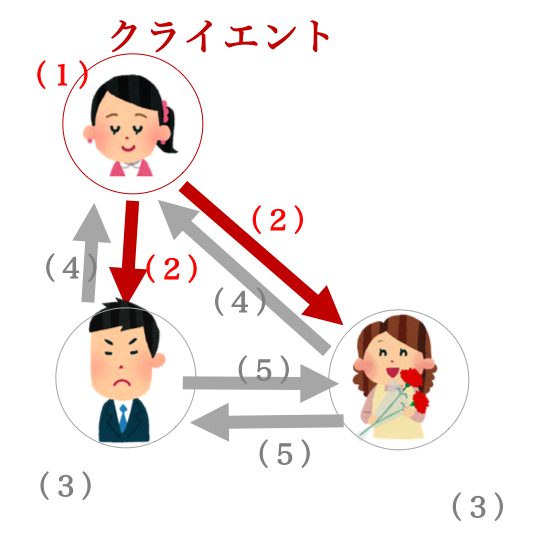
\includegraphics[width=\linewidth]{arrow.png}
  \end{center}
  \caption{認知の修正が進んでいる時に現れる矢印と進んでいない時に現れる矢印}
  \label{fig:arrow}
\end{figure}

\begin{enumerate}
  \item 「クライエント自身」の内的感情・「クライエントの周囲の人」に向けられていない「クラ
  イエント」一人の行動
  \item 「クライエント自身」から「クライエントの周囲の人」へのポジティブな行動


  \item 「周囲の人」の内的な陰性感情の予測や,他者に向けられていないその
  「周囲の人」一人のネガティブな行動
  \item 「クライエントの周囲の人」から「クライエント自身」へのネガティブな行動
  \item 「クライエントの周囲の人」から「クライエントの周囲の人」へのネガティブな行動

\end{enumerate}
上記のうち,1と2は「自己努力」,3,4,5は「状況依存」に分類される.

\section{要件抽出と実装}

% クライエントの認知補正の分析は,何らかの形でのように述べたクライエントの言動のカテゴリを使用 図.2 動作は,クライエントの周りの人々が行っていたものが挙げられる. 鎌田\cite{kamata2002}によると,カウンセラーの言動や感情を重要な役割は,クライエントが自己決意と自己責任を取ると不当に他人に介入することなく,他者との協力関係を形成することができるようにクライエントを奨励することである.だから,不当に他人の言動や感情に介入することなく,クライエント自身の言動や感情を見つけることが重要である.
%
%   カウンセリングで,「自分の言動を変えるのではなく,相手の言動を変えることに関心がある人は,認知を修正するに進んでいる」と言われている.ときに,クライエントの答え「クライエント自身の言動」ではなく答えるクライエントの認識の修正が進んでいると言われて, 『クライエントの周りの人々の言動を.』

\subsection{要件抽出}

図\ref{fig:arrow}をカウンセリングの会話文中の各タイミングにおいて描画するには、「会話文中のどのタイミングで誰が誰に対して言動をどれくらい発したか」の情報が必要である。「ある登場人物が別の登場人物に対して発した言動」、つまり、
\begin{itemize}
  \item 言動
  \item その言動の主語
  \item その言動の目的語
\end{itemize}
の関係をカウンセリングの会話文から得るには、カウンセリングの会話文に対して、後述する係り受け解析を行い、登場人物と動詞の係る―係られる関係を取得することが必要である。

また、「ある登場人物が別の登場人物に対して発した言動」がどれくらい行われているかは、図形の大きさや太さで表すものとし、それらが「会話文中のどのタイミングで」行われているかを可視化するためにはスライドバーが必要である。
以上を踏まえて、本システムでは次項に述べる前処理の実装を行った。



% 本研究における「クライエントの認知の修正に関する視覚的分析支援」では,「クライエント自身の言動」または「クライエントの周りの人の言動」について、「会話文中のどのタイミングで誰が誰に対して言動をどのくらい発したか」を可視化することにより,クライエントの認知の修正の評価を支援することを目的とする.本研究では時系列順に会話内容をテキストで言動の主語と目的語を可視化することにより,上記のニーズを満たすことができると考えた.




\subsection{前処理の実装}

本節では,「会話文中のどのタイミングで誰が誰に対して言動をどれくらい発したか」を可視化する人間関係図を生成するために本研究で行った,登場人物データと言動データを抽出する手法を説明する.テキストデータ内のオブジェクトデータ. 図\ref{fig:charaFlow}は,前処理の流れを示している.








\subsubsection{係り受け解析}


係り受け解析,または構文解析(syntactic analysis あるいは parse)とは,文章を,形態素に切分け,さらにその間の関連(修飾-被修飾など)といったような,統語論的(構文論的)な関係を図式化するなどして解析する手続きである.自然言語については自然言語処理における要点のひとつであり,プログラミング言語など形式言語の場合は,形式文法に従い構文木を得る.構文解析を行う機構を係り受け解析器(parser)と呼ぶ.



\subsubsection{登場人物と動詞の抽出}


本項では,文章中の登場人物を抽出する手法について説明して.カウンセリング会話書き起こしテキストデータをKNPに入力されたときに,このシステムの入力は,KNP \cite{KNP}(係り受け解析器)の出力結果である.次に,ある名詞(登場人物候補)「カテゴリ:人」を抽出した.元の文は,日本語形態素解析器JUMAN\cite{juman}によって分析される. JUMANは,形態素解析時に,独自の辞書によって,日本の各単語を分類する.したがって,JUMANにより「人」のカテゴリに分類された単語を抽出することにより,本研究では,文章中の文字を抽出した.

JUMANの品詞解析機能を用いて、カウンセリングの会話テキストから、登場人物と同様に「品詞:動詞」となっているものをリストアップした.また次項と次次項に向けて、各動詞の主語と目的語となる登場人物を把握することができるように、それぞれの動詞の周りの依存関係を把握するよう保存した.


% \subsubsection{動詞の主語と目的語の抽出}

\subsubsection{動詞の主語の抽出}


各動詞に係られる文節のうち,前節で「登場人物」に含まれる名詞の中で,

\begin{itemize}

  \item KNPにおいて,「私が」「Bさんが」等,<ガ格>として出力されたもの
\end{itemize}
に含まれるの名詞を,その動詞に対する名詞とした.

「私は」「Bさんは」等<ハ>で始まるものは,「Aさんは先生にこれをあげたい」の「Aさん」等,主語になるものと,「BさんはAさんがこれを上げた人だ」の「Bさん」等,目的語になるものがあるため,今回は無視した.

\subsubsection{動詞の目的語の抽出}


各動詞に係られる文節のうち,前節で「登場人物」に含まれる名詞の中で,

\begin{itemize}

  \item KNPにおいて,「私を」「Bさんを」等,<ヲ格>として出力されたもの
  \item KNPにおいて,「私に」「Bさんに」等,<ニ格>として出力されたもの
\end{itemize}
に含まれるの名詞を,その動詞に対する名詞とした.

\subsubsection{会話文中のどのタイミングで誰が誰に対して言動をどのくらい発したかのカウント}

その後,カウンセリング会話テキスト内で主語と目的語の同じペアを持っている動詞をカウントした.このカウントから、「会話文中のどのタイミングで誰が誰に対して言動をどのくらい発したか」がわかり,円や矢印が意味する動詞の数によって,後述する図\ref{dummyChara}のグラフに円の大きさや矢印のストローク幅に反映されている.

%%%%%$ 認知の修正可視化結果

\section{可視化}

本節では,我々の提案した「クライエントの認知の修正評価支援システム」の可視化部分について説明する.この「クライエントの認知の修正評価支援システム」における可視化結果の図\ref{fig:dummyChara}に示す.可視化結果は,「人間関係図」「スライドバー」「原文表示ビュー」3つの項目から構成されている.本研究では,可視化のためにD3.js\cite{vand3}を使用した.%それが書かれた書き起こし産物に基づきる.

\begin{figure}
  \begin{center}
    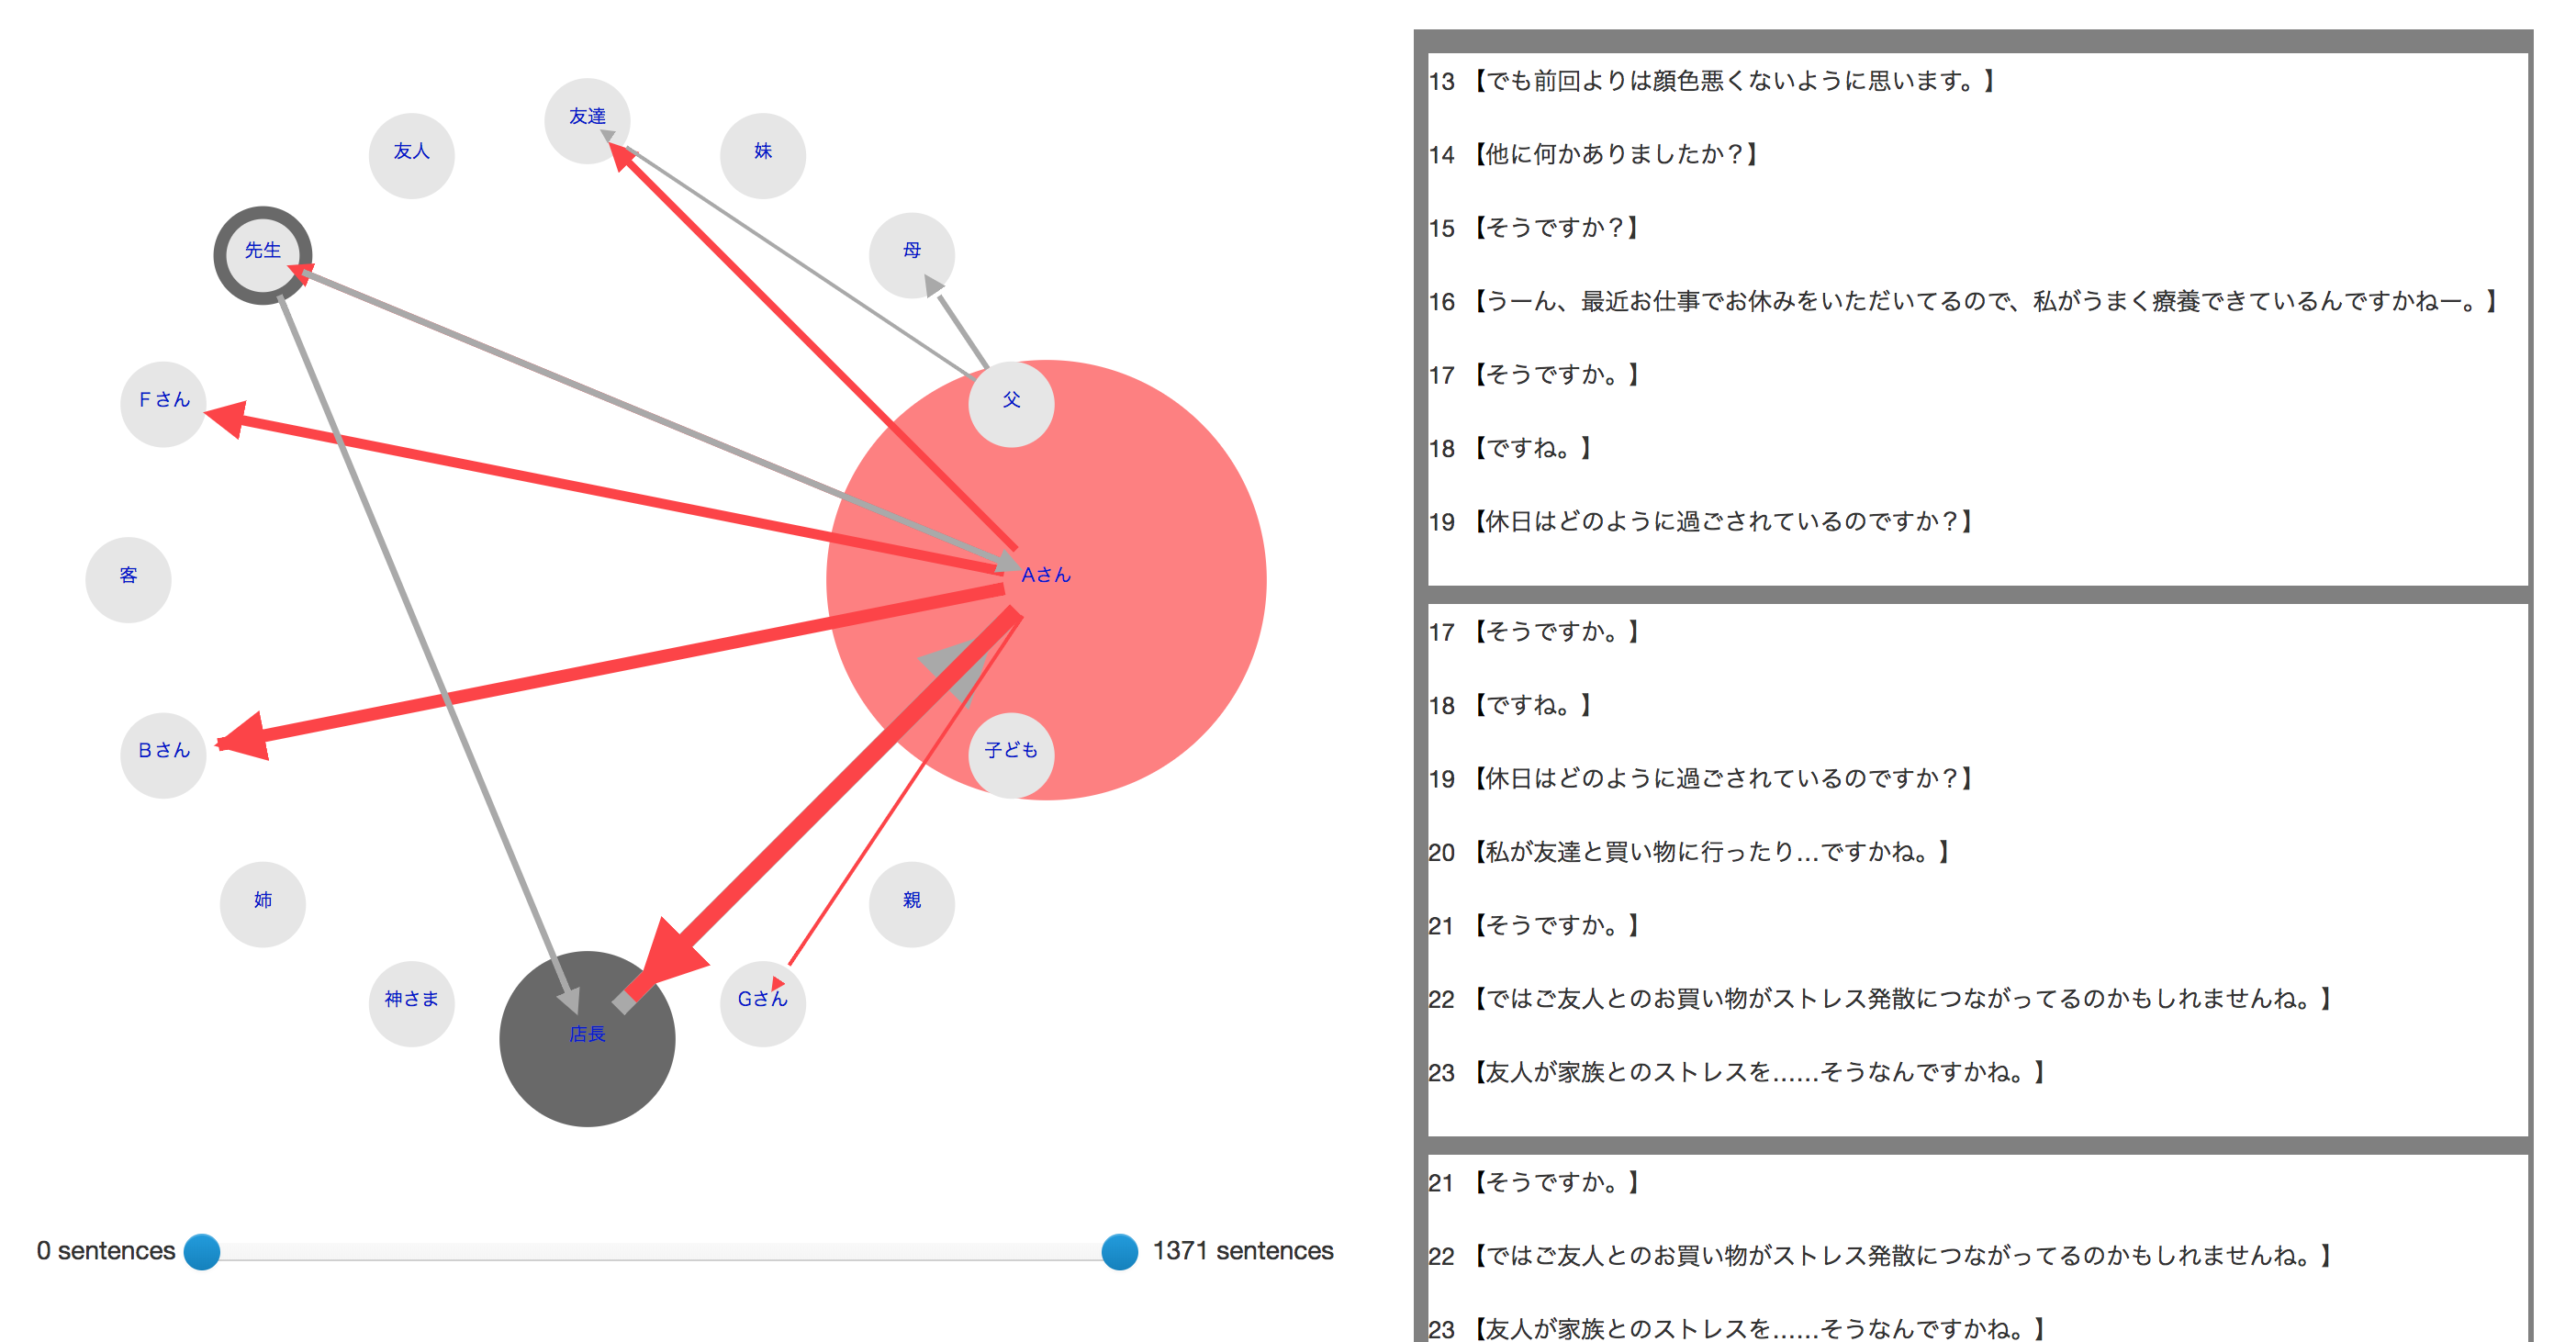
\includegraphics[width=\linewidth]{dummyChara.png}
  \end{center}
  \caption{「クライエントの認知の修正評価支援システム」の可視化結果(ダミーデータ)}
  \label{fig:dummyChara}
\end{figure}

\subsection{人間関係図}

ヴァンハムら\cite{van2009mapping}は文章を分析し,"B of A"および"A and B"の関係を有向グラフで表現した.しかし本研究では、「会話文中のどのタイミングで誰が誰に対して言動をどのくらい発したか」を有向グラフで可視化した。

田中ら\cite{tanaka}は効率的に話の内容を想起するためのインタフェースを開発した.しかし,彼らは登場人物ではないものを含め,頻繁キーワードを可視化する.また,彼らはそれがどのようなシーンで起こったことかを可視化を行っていない.

田中らは無向グラフによる可視化であったが,本研究では色分けされた有向グラフによって,カウンセリングの会話テキスト内の人間関係図を可視化することで,認知の修正の分析の支援を行う.

\subsubsection{会話文中の登場人物の内的感情や一人で完結した言動を表す円形}

カウンセリングの会話文内に登場する人物が円周上に一覧として並べられ,その会話中でその人物が起こし,目的語を持たない言動の数は,円の大きさで表されている.クライエント自身であれば円はピンク,それ以外は水色で表している.鎌田\cite{鎌田穣2002臨床}が提唱した図\ref{fig:arrow}において、
\begin{itemize}
  \item ピンクの丸……「クライエント自身」の内的感情・「クライエントの周囲の人」に向けられていない「クライエント」一人の行動
  \item 水色の丸……「周囲の人」の内的な陰性感情の予測や,他者に向けられていないその
  「周囲の人」一人のネガティブな行動
\end{itemize}
を表している。したがって、ピンクの丸がより大きくなれば認知の修正が進行していると判断する。

\subsubsection{会話文中の登場人物が別の登場人物に対して行った言動を表す矢印}

矢印は「誰か」から「誰か」への言動の発生を表している.
矢印の直線の太さで,その言動の数を表現している.
前節でカウントした,「主語・目的語の組み合わせが同じ動詞」を1つの「矢印」にまとめ,その「動詞」の数を「矢印」の太さで表現している.


\begin{itemize}
  \item 「クライエント自身」から「クライエントの周囲の人」へのポジティブな言動:(「ネガティブだが,もしもの話」の場合を含む)→赤の矢印
  \item 「クライエント自身」から「クライエントの周囲の人」へのネガティブな言動:(「ポジティブだが,もしもの話」の場合を含む)→青の矢印
  \item 「クライエントの周囲の人」から誰かへのポジティブな言動:(「ネガティブだが,もしもの話」の場合を含む)→オレンジの矢印
  \item 「クライエントの周囲の人」から誰かへのネガティブな言動:(「ポジティブだが,もしもの話」の場合を含む)→緑の矢印
\end{itemize}

したがって、赤やオレンジの矢印が多くなったり太くなったりするほど、認知の修正が進行していると判断する。

\subsection{スライドバー}

カウンセリングの会話の原文のうち,200文分を上記グラフにて可視化している.初期表示では0文目〜200文目についてのグラフを表示している.

青丸にマウスカーソルを合わせると,いま何文目から何文目までについての可視化を行っているか,吹き出しで表示される.
青丸を動かすことで,可視化する会話文の範囲を変えることができる.


\subsection{原文表示機能}

グラフの登場人物の円をクリックすると,「その登場人物が登場するカウンセリングの原文箇所」が,画面右側に表示される.
グラフの矢印をクリックすると,右側に「その矢印に該当する言動を示すカウンセリングの原文箇所」が,画面右側に表示される.
原文表示で下線が引かれている場所に,そのクリックした矢印に該当する動詞が含まれている。


\section{ユーザー評価と考察}

\subsection{ケーススタディ}

同じカウンセラー・クライエント同士で行われた5回分の実際のカウンセリングテキストデータを時系列順に並べ,1つのテキストデータとした.このテキストデータKNPで係り受け解析した後,その係り受け解析結果を我々が提案した「クライエントの認知の修正評価支援システム」に入力し,可視化手続きを行った.

図\ref{fig:caseFirst}のように,最初2回のカウンセリングの辺りでは,クライエントである「Aさん」自身が行った「Bさん」に対するネガティブな言動が目立った.しかし,図\ref{fig:caseSecond}のように,「Bさん」だけでなく「店長」に対するクライエント自身のネガティブな言動をクライエントが言及するようになったことがわかった.そして5回目のカウンセリングでは,図\ref{fig:caseThird}のように,クライエント自身から「店長」へのポジティブな言動が目立つようになった.


\begin{figure}
  \begin{center}
    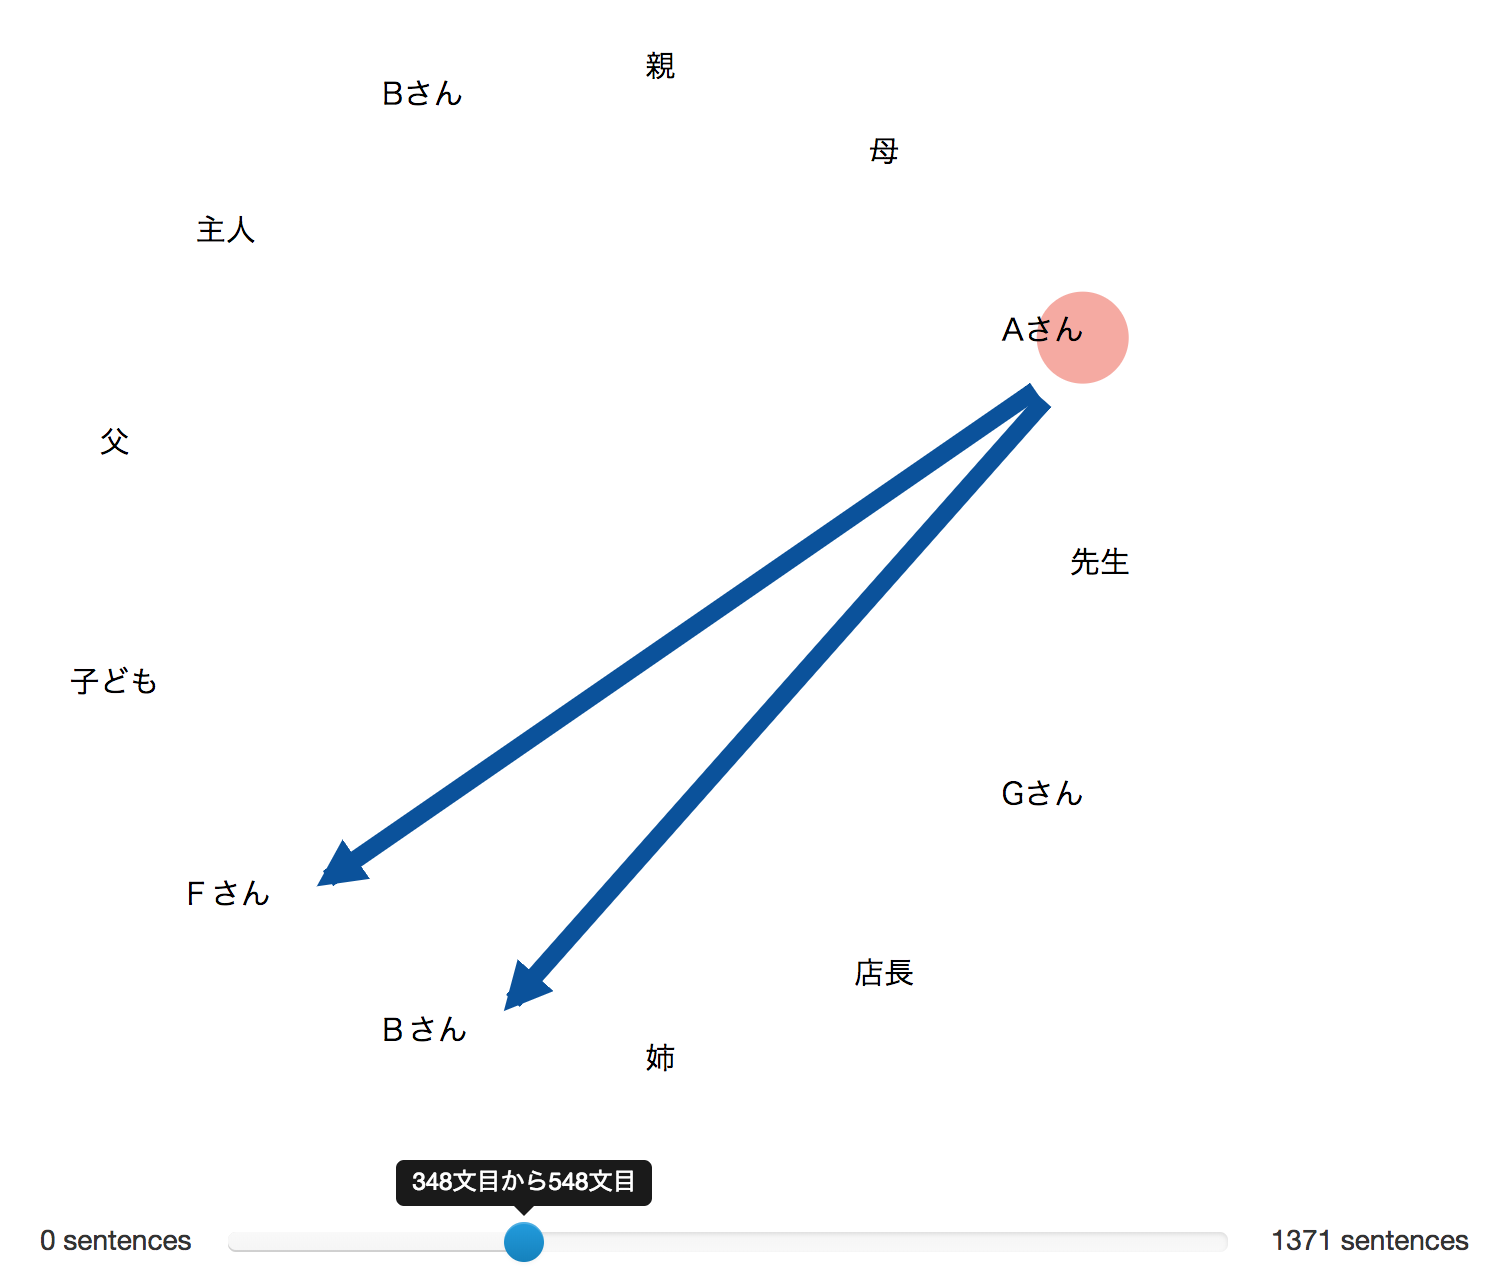
\includegraphics[width=\linewidth]{caseFirst.png}
  \end{center}
  \caption{ケーススタディ348文目から548文目における可視化結果}
  \label{fig:caseFirst}
\end{figure}

\begin{figure}
  \begin{center}
    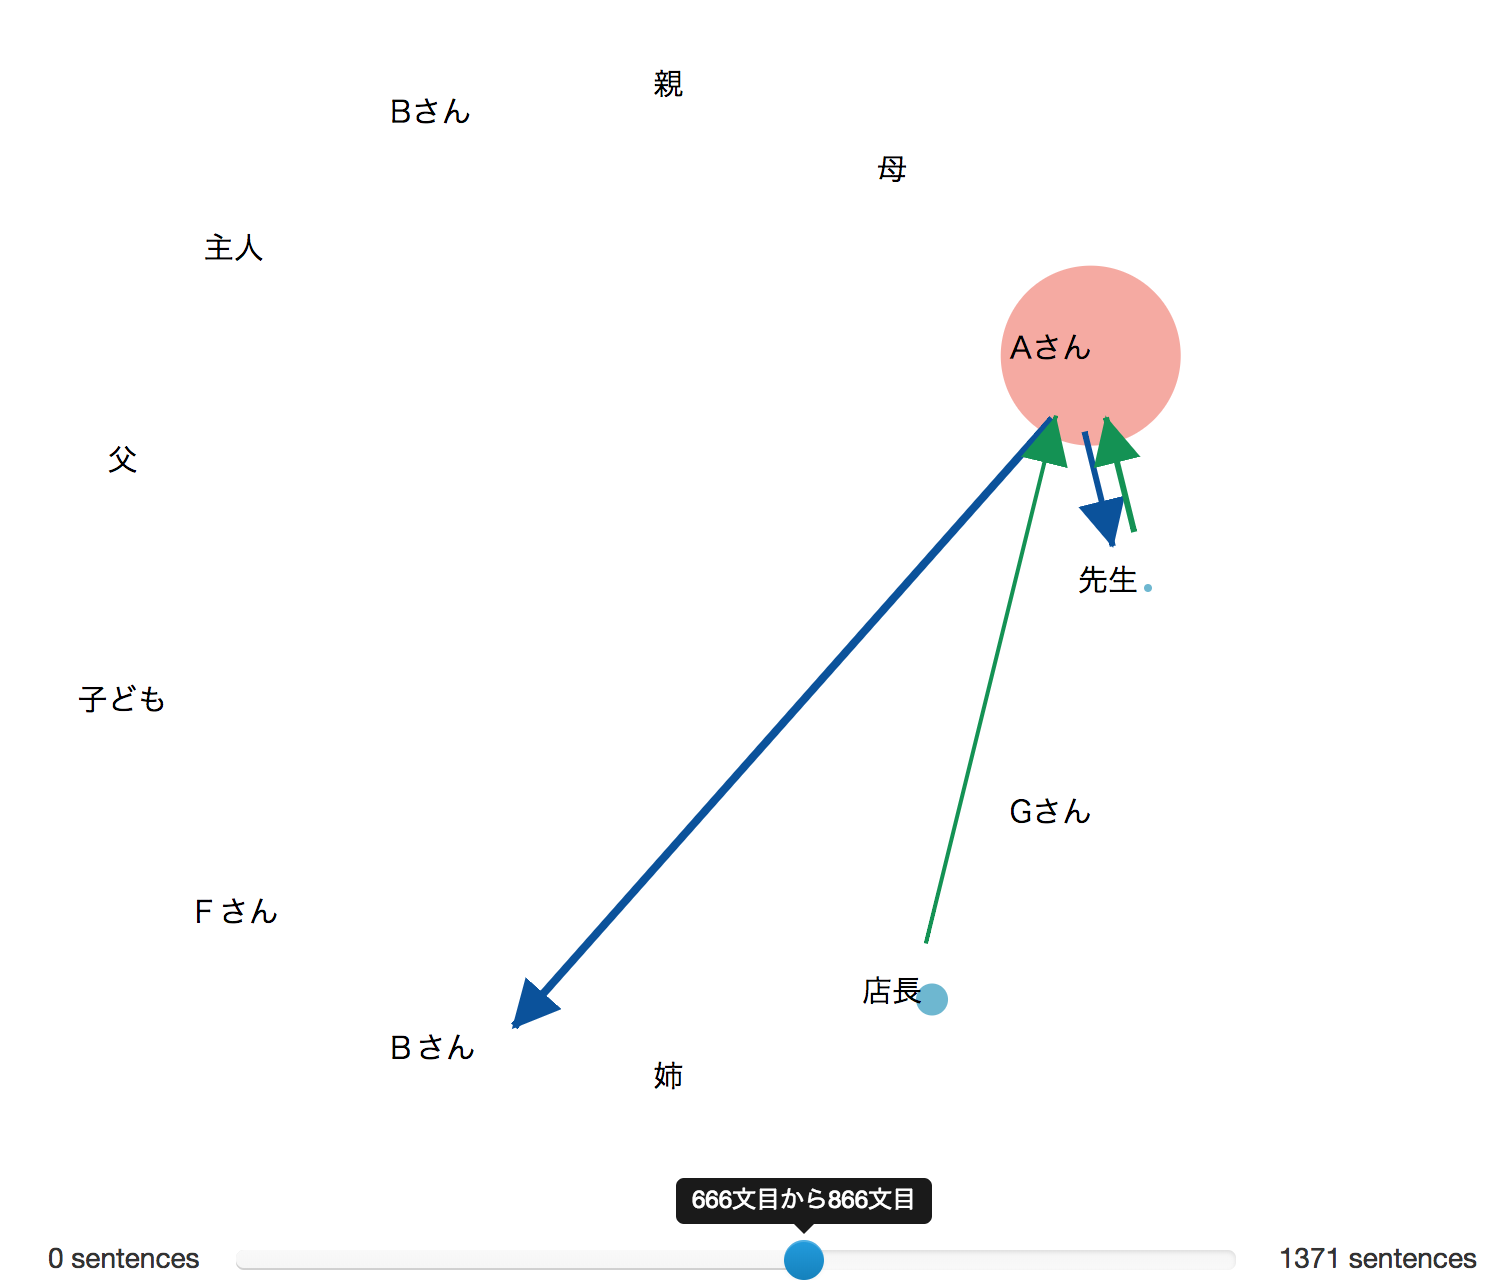
\includegraphics[width=\linewidth]{caseSecond.png}
  \end{center}
  \caption{ケーススタディ666文目から866文目における可視化結果}
  \label{fig:caseSecond}
\end{figure}

\begin{figure}
  \begin{center}
    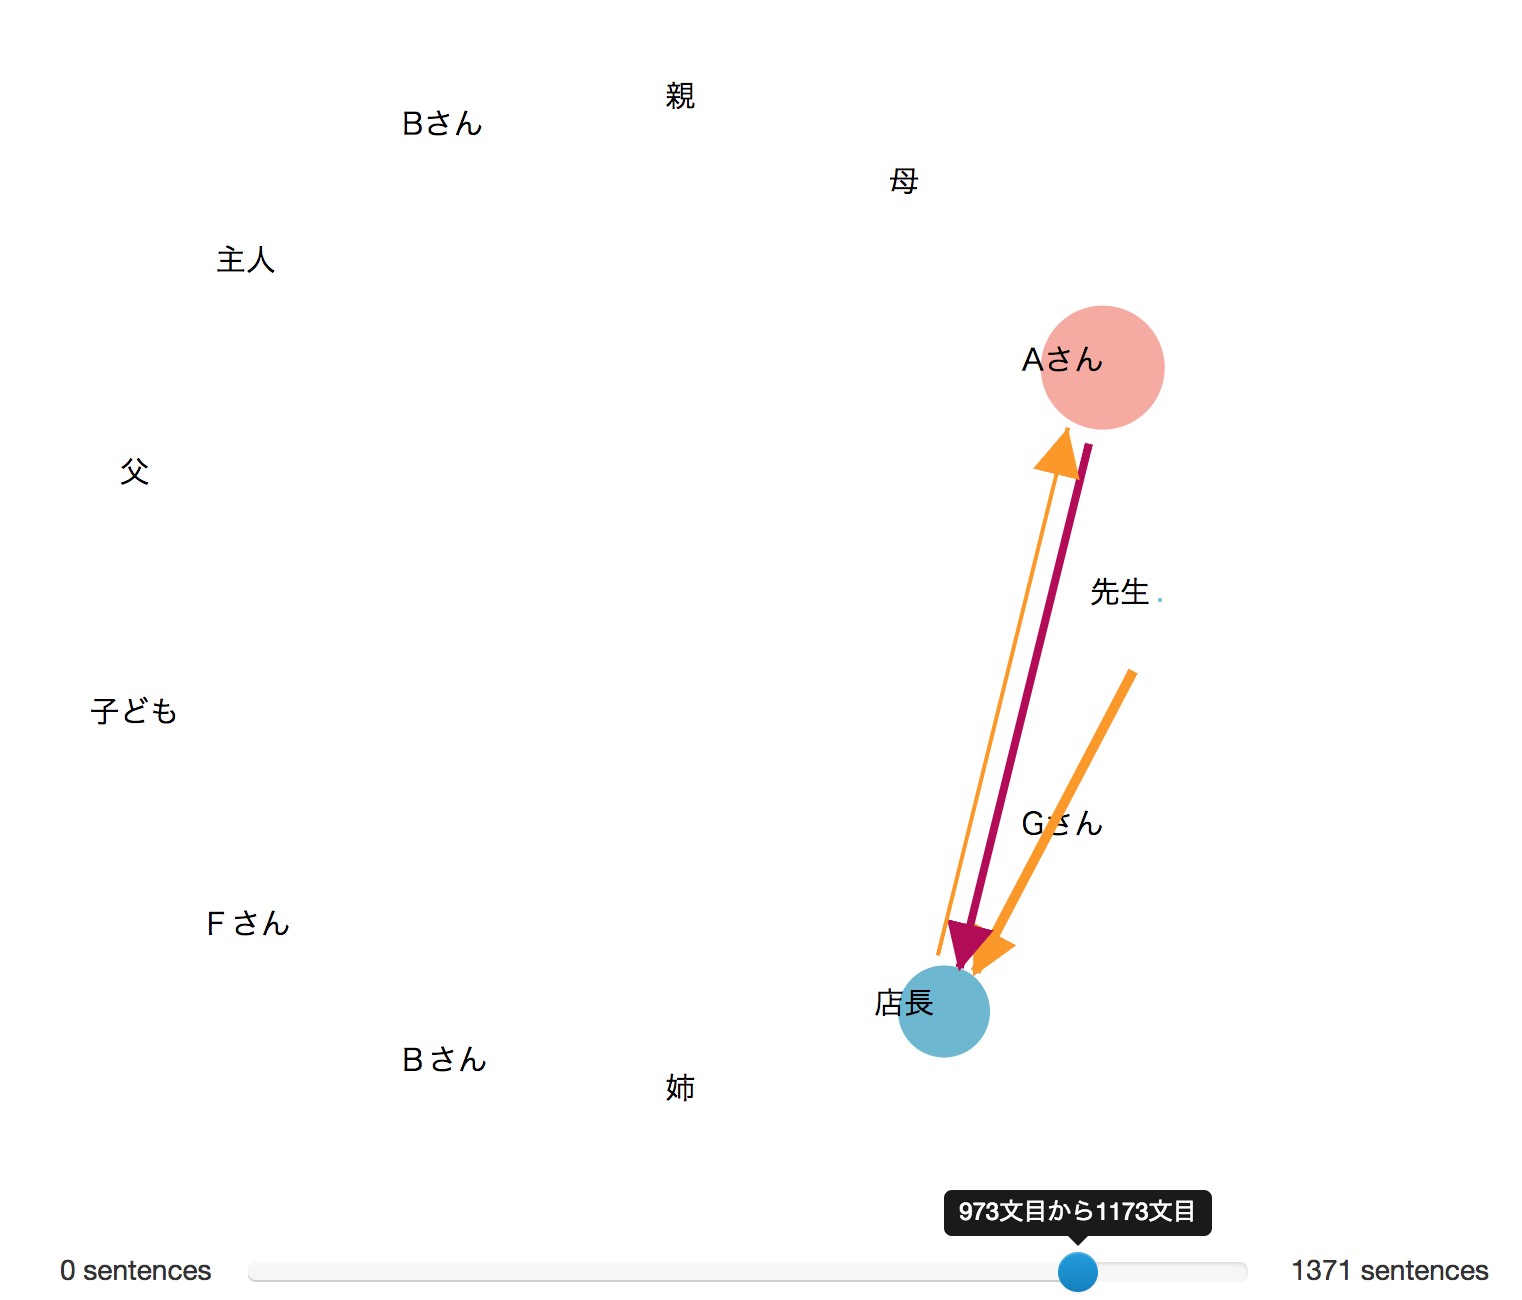
\includegraphics[width=\linewidth]{caseThird.png}
  \end{center}
  \caption{ケーススタディ973文目から1173文目における可視化結果}
  \label{fig:caseThird}
\end{figure}

% The expert counselor said that he found out that the idea "I want B to follow my will" disappeared
and self-closed task increased. Progress of correction of cognition could be confirmed by changing the quantity of arrows (Overall view of multiple counseling) and confirming the quality in original text display. We consider that our proposed character chart visualization helps counselors find out that some kind of client's cognitive fixes were made.
%
% 図1カウンセリング1
% 図2カウンセリング2

\subsection{エキスパートコメントと考察}

前節のケーススタディの可視化結果を出力した本システムについて,矢印の色分けをなくしたものと色分けを施したものの2パターンについて熟練したカウンセラー1名に見ていただき,エキスパートコメントを得た.まず
\begin{enumerate}

  \item 「私がBさんを思い通りにしたい」というような
  自分で閉じた話題「セルフタスク」への変化がみてとれた.
  \item クライエントから店長に向かっている矢印が増えた。
  \item 複数のカウンセリングの全体俯瞰をすることで、矢印の量の変化が確認できた。
  \item 原文表示での質の確認により,認知の修正の進行が確認できた。
\end{enumerate}
というコメントが得られた.中盤になって「クライエント自身」の内的感情・「クライエントの周囲の人」に向けられていない「クラ
イエント」一人の行動,すなわちセルフタスクが増えたことで,認知の修正の評価を支援できたと考えられる.
また,「色付きの方がネガティブとポジティブについてわかりやすい」というコメントを得た.ポジティブかネガティブかを可視化することで,単なる矢印よりもさらにできることが考察できる.


「
赤とオレンジの増加が最後は認められ,このあたりから認知の修正の可能性が
認められるようになったと考えます.クライエントほんにんの内的感情状態がネガティブなのかポジティブなのかが
わかるようになると大変役立つと思いました.大きさだけでは,ネガティブかど
うかがわからないところです.こうやって,全体の流れが見えると,かなりみやすくなってきたように思いま
す.
」といったコメントが得られた

矢印の分類の信憑性の問題は,テキスト分析の問題なので,今後の課題であると考える.







\begin{itemize}

  \item 矢印の意味合いが違えど,何かしらの認知の修正があったことはツールから分かった
  \item 「感謝・貢献」と「悪いアイツかわいそうな私」を言語処理で分別するのは厳しい

  \item せめてその2種類を手動修正して区別して提示することで,他のカウンセラーに説明しやすくすべき

\end{itemize}
%%%結論
\chapter{結論}

本章では,本研究における結論,および,本研究で述べた内容の将来性について述べる.

\section{結論}

本研究では,時間軸に沿った可視化によって,クライエントとカウンセラーの会話の流れを可視化するWebシステムを開発したが,本研究では特に,
\begin{itemize}
  \item 「事例検討会通りに原文を読んでカウンセリングを評価すること」との対比
  \item 新たなチャート可視化の提案と,既存チャート可視化との対比
\end{itemize}
について述べた.熟練したカウンセラーから初心者へのカウンセリング指導において,どのような質問を初心者のカウンセラーがクライエントに投げかけるかによって,初心者のカウンセラーがクライエントからどのような「対人関係上の問題」に関する回答が発せられたかが重要である.それが一目見てわかるようになったことが,本システムにて実現されたことであると,「事例検討会通りに原文を読んでカウンセリングを評価すること」との対比から結論付けられる.また,特にこの実現について寄与するものであると筆者が考えるのは,縦棒同士の間隔が等間隔であるグラフデザインよりも,縦棒同士の間隔のクライエントの発言の文字数に比例するグラフデザインであることが,本研究で述べた「新たなチャート可視化の提案と,既存チャート可視化との対比」から裏付けられたと考える.会話の流れの可視化システムは,カテゴライズを変えることによって,例えば就職の面接のインタビューにおける人事部社員の教育・反省など,カウンセリング以外の用途に適用されることが期待できる.

% しかし前章で述べたとおり,本システムのWeb上での描画所要時間は今後検証しなければならない.初心者のカウンセラーを指導する目的で本システムを実用化するには,まだまだ視覚的表現やユーザーインタラクションについて議論すべきタスクが残されている.次節で今後の課題についてまとめる.


%本提案システムのユーザーとして想定している熟練したカウンセラーからは「この研究が進んでいくことによって,心理臨床におけるスーパーヴィジョンにおいて,客観性にもとづく指導が可能になって
%いけることを願っておりる.こういう着想はありないでしたので,大変期待
%しているところである」
%という本研究への評価を得た.

% 本論文で,本研究ではまず,それが会話の流れが正常に全体として新しいカウンセラーに指針を与えるために可視化された複数の経験豊富なカウンセラーからの回答によって裏付けられていることを結論付けている.本研究で提案した帯グラフは,カウンセリングでの会話の流れの可視化で,積み重ね折れ線グラフを超える新しいカウンセラーの指導に優れたチャートになっていると結論付けられる.

%  また,目的語を可視化し,矢印でテキスト内の言動の情報を目的語によって,それは「クライエントの周りの人の言動を可視化」かによって,データを可視化することが可能となる「クライエント自身の言動を.」

また本研究では,カウンセラーが言動矢印の付いた人間関係チャートの提案時系列可視化によって認知の修正の状態を確認できることが示唆されたと結論付ける.矢印の色付けされた有向グラフの人間関係図を使用していつどの方向の言動が置きているかを可視化する手法は,このような新規のシーンを把握などのテキスト内の文字の時系列推移を確認するために,例えば,小説や映画スクリプトの可視化など,カウンセリング以外の分野にも適用することができると考えられる.我々の提案するシステムは,言語処理の言語を返すことによって,英語など,日本語以外の言語にも適用することができる.

以上から、本研究で提案したこの2つの可視化システムによって、本研究内で定義した心理カウンセリングにおける品質の向上の支援ができることを示唆できたのではないかと結論付ける。これらの可視化を用いて、上記に述べたような心理カウンセリング以外のテキストデータに対しても応用が可能ではないかと考える。


\section{今後の課題}

本研究で得られたことを踏まえて,今後検討するべきタスクを簡単にまとめる.

まず

\begin{itemize}
  \item 熟練したカウンセラー達の間でカウンセリング内容の共有が効果的に行えるようになるかの検証
  \item ConTovi\cite{el2016contovi}など,話題の可視化に関する,他のグラフ描画手法との比較
  %\item 本提案システムの縦軸や横軸のスケールの取り方
  %  \item 縦棒の上に発言番号を振ること「自己」と「スピリチュアル」のグループの追加
  \item ブルーライトカットのディスプレイなどを使用しているユーザーが色を見分けにくいなどの理由から,本提案システム全体の配色面に関しての改善
  %  \item ユーザー側で最初から最後まで簡単に可視化を行うために,カウンセリングを書き起こしたテキストデータを自動で本システムの入力データフォーマットとなる会話データに変換する機能の搭載
  %  \item 本システムのユーザーのカウンセラーに,入力する書き起こしテキストデータの文章量が多いと積み重ね折れ線グラフの縦棒が密集してしまう問題を解決するために,全体の積み重ね折れ線グラフから一部分を抜き出して描画するズーム機能
  %  \item ユーザーから見た本提案システムの視覚的表現やユーザーインタラクションについての定量的な評価
\end{itemize}

初心者のカウンセラーを指導する目的で本システムを実用化するために,以上の今後の課題について取り組むことが求められる.%\cite{Nielsen}

\subsubsection{クライエントの認知の修正評価支援システム}

今回実装が間に合わなかったが,まず照応解析\cite{sasano2009probabilistic} \cite{sasano2011discriminative}を用いた,「彼」「彼女」などの代名詞で表された登場人物のカウントが,言動検出精度向上には必要である.また
\begin{itemize}
  \item 談話解析をすることによるif文の取得\cite{kishimoto}
  \item その単語がネガティブかポジティブかを判定する辞書を用いた,矢印の自動分類機能\cite{小林のぞみ2005意見抽出のための評価表現の収集} \cite{東山昌彦2008述語の選択選好性に着目した名詞評価極性の獲得} の導入
\end{itemize}
を用いた,矢印で表された言動の自動分類が求められる.

評価の点においては,田中ら\cite{tanaka}のような無向グラフ人間関係図との比較が求められる.

また、本研究で提案した「カウンセラー習熟度評価支援システム」と「クライエントの認知の修正評価支援システム」という2つのシステムを同時に可視化することで、「カウンセラー習熟度」と「クライエントの認知の修正」の互いの可視化結果を他に生かせるのではないかとも考えている。しかし両システムを1つの画面に移すには省スペース化などの工夫が必要であると考える。




%======================================================================
%		謝辞
%======================================================================
\begin{acknowledgements}
  この度の事例データ提供についてご快諾いただきた事例提出者ならびにクライエントご本人,そして研究支援を惜しみなく行っていただいている(社)日本ヨーガ療法学会理事長木村慧心先生に深く感謝いたします.

  本研究を進めるにあたり,提案システムへの助言,システム評価などに協力して下さった,臨床心理士の鎌田穣先生にはご協力を賜りた.ここに深く御礼申し上げます.また,我々の提案システムをご評価いただいたスーパーヴァイジーの皆様・スーパーヴァイザーの皆様に深く御礼申し上げます.

  その他,2016年1月提案システムのプロトタイプ以降,定期的に本研究に対して意見をくださった「心の可視化研究会」参加者の皆様にも深く感謝致します.

  本研究を進めるにあたり,有益な御指導,御助言を頂きた京都大学学術情報メディアセンタービジュアリゼーション研究分野の小山田耕二教授,江原康生准教授をはじめ,小山田研究室の皆様に深く感謝致します.



  %本研究を進めるにあたり,プログラミング技術を始め,様々な御助言を頂きた京都大学大学院工学研究科博士後期課程3年生の尾上洋介氏,京都大学大学院人間・環境学研究科修士課程1年生の今井晨介氏をはじめとする院生の先輩の皆様に深く感謝致します.

  最後に,家族をはじめとする私の学生生活を支えてくださったすべての皆様へ心から感謝の意を表します.
\end{acknowledgements}



%======================================================================
%		参考文献
%======================================================================
\bibliographystyle{kueethesis}
\bibliography{sotsuron}



%======================================================================
%		付録
%======================================================================
% \appendix
% \chapter{アンケート項目について}
% 	あなたが,ラクロスの試合,練習を分析し,戦術,試合,練習を改善する立場にいる(チームの分析,自分個人の分析)と考えて回答してください.
% 	\begin{itemize}
% 		\item どういった表現手法で見せて欲しいか.
% 			今のイントラ表現と比較して答えてください.「〜」表現手法.(いくつ選んでもok)
% 			\begin{itemize}
% 				\item 他人と,他チームと比較がしやすい.
% .
% 				\item 時系列で見れる.
% 			\end{itemize}
% 		\item その他,上にない表現手法で,要望となるようなものがあれば書いてください.
% 		\item 分析をする際に欲しい情報は何か.
% 			「〜」に関すること.(いくつ選んでもok)
% 			\begin{itemize}
% 				\item ラントレ
%
% 			\end{itemize}
% 		\item その他,上にない欲しい情報があれば書いてください.
% 		\item ラクロスの様々なデータが見やすくなったとする(可視化された).あなたならどういったシチュエーションで可視化ツールを使いるか
% 	\end{itemize}
%
%
% \chapter{本提案システム評価アンケート}
% 	\begin{itemize}
% 		\item 本提案システムの利用について
% 			\begin{enumerate}
% 				\item 使用不可:実際の現場で実用する依然に使用するのが困難である.
%
% 			\end{enumerate}
% 		\item 表計算ソフトの利用について
% 			\begin{enumerate}
% 				\item 使用不可:実際の現場で実用する依然に使用するのが困難である.
%
% 			\end{enumerate}
% 		\item 本提案システムは利用用途に沿っているか
% 			アンケート項目より,回答に多かった利用用途は「対戦相手チームの特徴を把握し,自チームの戦術を練るため.」「試合後に,自チームの反省を行ない,以後の方針を決定するため.」「結果の良かったエレメントと,悪かったエレメントの違いを見出し,新たな視点を得るため.」「試合に出るレギュラーを選定する材料とするため.」「データの蓄積を行うことで,最適な戦術を選び出すため.」
%
% 	\end{itemize}


%\chapter{男子ラクロスについて}



\end{document}
% Local Variables:
% fill-column: 70
% End:
